% !TEX root = ./thesis-main.tex

% !TEX root = ../thesis-main.tex

\RequirePackage{mathtools}  % mathtools asks to be loaded before unicode-math...
\documentclass{kthpq-thesis}

% ==== PACKAGES ====

% ---- kthpq-thesis ----

% Custom biblatex package to have cool macros
\usepackage[%
  bibstyle=numeric,
  maxnames=99,
  isbn=false,
  url=false,
  urldate=ymd,
  defernumbers=true
]{biblatex-kthpq}

% \makeatletter  % bibliography numbers in margin...
% \defbibenvironment{bibliography}
% {\list{\printtext[labelnumberwidth]{%
%     \printfield{prefixnumber}%
%     \printfield{labelnumber}}}
% {\setlength{\bibhang}{0pt}%
% \setlength{\leftmargin}{\bibhang}%
% \setlength{\itemindent}{-\leftmargin}%
% \setlength{\itemsep}{\bibitemsep}%
% \setlength{\parsep}{\bibparsep}}}
% {\endlist}
% {\item}
% \makeatother

% ---- Formatting ----

\usepackage{parskip}

\usepackage[
  % demo  % omit inclusion of PDFs
]{pdfpages}

% longtable: ignoring this error https://github.com/latex3/latex2e/issues/1907
% with VS Code LaTeX Workshop 
\usepackage{longtable}

% ---- Math ----

% mathtools loaded at the top!
\usepackage{amsthm,thmtools}  % thmtools for QED in any theorem

% ---- Floats ----

% \usepackage{flafter}
\usepackage{caption}
\usepackage{subcaption}

% ---- Other ----

\usepackage{tikz}
\usetikzlibrary{babel,calc,cd}
\usepackage[ruled]{algorithm2e}

\usepackage{imakeidx}

% ---- Load last ----

% Hyperref needs to come after parskip
% (https://tex.stackexchange.com/questions/450551/theorems-and-parskip#comment1853746_450551),
% and generally should be loaded last.
\usepackage[
%  draft, % Uncomment to remove all links (useful for printing in black and white)
%  hidelinks,
  % bookmarksdepth,% w/o argument: uses tocdepth, supposedly
  pdfusetitle,
  colorlinks,
  linktoc=all,
  allcolors={digital blue}
]{hyperref}

% amsmath (from unicode-math) > hyperref > cleveref
\usepackage[noabbrev,capitalize]{cleveref}

% ==== COMMANDS ====

% \WarningFilter{latex}{Marginpar on page}
\DeclarePrintbibliographyDefaults{title=References}

% ---- Font ----

\setmainfont{Georgia Pro}[
  Uprightfont = *-Regular,
  BoldFont = *-Bold,
  ItalicFont = *-Italic,
  BoldItalicFont = *-BoldItalic,
  Numbers = OldStyle,
  Scale = \fontscale
]

% ---- Proofing ----

% \geometry{showframe}  % layout frames
% \usepackage{lua-visual-debug}  % more boxes!
% \overfullrule=10pt  % visual indicator of overfull boxes

% ---- Bibliography ----

\addbibresource{bib/mine.bib}
\addbibresource{bib/kappa.bib}
\addbibresource{bib/CI.bib}

\DeclareFieldFormat{eprint:github}{%
GitHub: \href{https://www.github.com/\strfield{eprint}}{\texttt{\strfield{eprint}}}
}

% ---- Layout ----

% Custom header and footer with fancyhdr
\fancypagestyle{fancy}{%
  \fancyhead{}  % reset
  \fancyhead[LO]{\sffamily\small\rightmark}
  \fancyhead[RE]{\sffamily\small\leftmark}
  \fancyhead[LE,RO]{\sffamily\small\thepage}  % Left for even pages, right for odd pages
}

\fancypagestyle{plain}{% for special pages, e.g. first pages of chapters
  \fancyhead{}  % reset
  \fancyhead[LE,RO]{\sffamily\small\thepage}  % Left for even pages, right for odd pages
}

\makeatletter
% Flipbook stuff: inspired by nilsvu/latex-flipbook on GitHub
% Current hunch is that pgfpicture sets the bounding box based on the vertices (the last path?)
\newif\if@frontmatter
\fancyfoot{}  % reset footer
\fancyfoot[RO]{%
  \if@mainmatter%
    \ifnum\thepage<60\relax%
      \AddToHookNext{shipout/background}{\put(\paperwidth-30mm,3mm-\paperheight){\input{figs/flip/leo-\fpeval{trunc((\thepage - 1) / 2, 0)}.pgf}}}%
    \fi%
  \else%
    \if@frontmatter%
      \AddToHookNext{shipout/background}{\put(\paperwidth-30mm,3mm-\paperheight){\input{figs/flip/leo-0.pgf}}}%
    \fi%
  \fi%
}

% Remove fancy headers from front matter and add check for front matter
\let\oldfrontmatter\frontmatter
\let\oldmainmatter\mainmatter
\let\oldbackmatter\backmatter
\def\frontmatter{\oldfrontmatter\@frontmattertrue\pagestyle{plain}}
\def\mainmatter{\oldmainmatter\@frontmatterfalse\pagestyle{fancy}}
\def\backmatter{\oldbackmatter\@frontmatterfalse}
\makeatother

\setcounter{tocdepth}{1}

% Try to make things more compact
%\linespread{.9}

% ---- Sections & titles ----

\newcommand{\inleftmargin}[2][\marginparsep]{%
  \makebox[0pt][r]{#2\hspace{#1}}%
}

\titleformat{\section}
  {\sffamily\fontsize{13pt}{13pt}\selectfont\bfseries}
  {\inleftmargin{\thesection}}{0em}{}

\titleformat{\subsection}
  {\sffamily\fontsize{12pt}{12pt}\selectfont\bfseries}
  {\inleftmargin{\thesubsection}}{0em}{}

% New section-like for papers
\makeatletter
\newcommand\papersection[2][]{% OPTIONAL: shorttitle, misctext
  \setkeys{kthpq@papersection}{#1}%
  \@papersection{#2}%
  \let\@misctext\defaultmisctext%
  \let\@shorttitle\@nil
}

\let\@shorttitle\@nil
\define@key{kthpq@papersection}{misctext}{\def\@misctext{#1}}
\define@key{kthpq@papersection}{shorttitle}{\def\@shorttitle{#1}}

\DeclareCiteCommand{\@papersection}
{%
  \pagetrackerfalse%
  \citetrackerfalse%
  \usebibmacro{prenote}%
  \defcounter{maxnames}{99}%
  \sffamily%
  \let\theoldsection\thesection
  \renewcommand{\thesection}{\papername\ \Alph{section}}
}
{%
  \ifx\@shorttitle\@nil
    \section{\thefield{labeltitle}}
  \else
    \section[\@shorttitle]{\thefield{labeltitle}}
  \fi
  % % automatically add label (outside labels don't detect this section)
  % \label{PS:\strfield{entrykey}}
  \printnames{author}.
  \ifentrytype{article}{%
    In \usebibmacro{tryfjournal},
  }{}%
  \ifentrytype{inbook}{%
    In \printfield{booktitle},
  }{}%
  \ifentrytype{incollection}{%
    In \printfield{booktitle},
  }{}%
  \ifentrytype{inproceedings}{%
    In \printfield{booktitle},
  }{}%
  \ifentrytype{misc}{%
    \@misctext\ifx\@misctext\empty\else, \fi%
  }{}%
  \printfield{year}.
  \printfield{doi}\printfield[eprint:arxiv]{eprint}%
}
{}
{%
  \usebibmacro{postnote}%
  \let\thesection\theoldsection
}

% Adding bibliographic data to ToC
% can't patch this command for some reason so here's the full thing
\renewcommand{\papertitlepage}[2][]{%
  \cleardoublepage%
  \newgeometry{top=30mm,bottom=30mm,left=43mm,right=\@tabmargin}%
  \thispagestyle{empty}%
  \setkeys{kthpq@papertitlepage}{#1}
  \phantomsection
  \paper@tab% before stepping counter for better positioning
  \refstepcounter{paper}
  \@papertitlepage{#2}
  \renewcommand{\thechapter}{\thepaper}
  \markboth{}{}% Reset header
  \addtocontents{toc}{%  <-- inserted block here
    \protect\def\protect\@misctext{\@misctext}%
    \protect\@paperdetailsintoc{#2}%
  }% end inserted block
  \let\@misctext\defaultmisctext
  \restoregeometry
  \vfil\newpage\null
  \thispagestyle{empty}
  \afterpage{\nopagecolor}% Reset the color after the current page
  \newpage
}

\def\@paperdetailsintoc#1{%
  \hspace{\cftchapnumwidth}%
  \parbox[t]{\dimexpr\textwidth - \cftchapnumwidth - \@tocrmarg\relax}{%
    \sffamily\@paperdetailsintoc@i{#1}
  }%
  \vspace{5pt}% manually adjusted
}

\DeclareCiteCommand{\@paperdetailsintoc@i}
  {%
    \pagetrackerfalse%
    \citetrackerfalse%
    \defcounter{maxnames}{99}%
  }
  {%
    \printnames{author}.
    \ifentrytype{article}{%
      In \usebibmacro{tryfjournal},
    }{}%
    \ifentrytype{inbook}{%
      In \printfield{booktitle},
    }{}%
    \ifentrytype{incollection}{%
      In \printfield{booktitle},
    }{}%
    \ifentrytype{inproceedings}{%
      In \printfield{booktitle},
    }{}%
    \ifentrytype{misc}{%
      \@misctext\ifx\@misctext\empty\else, \fi%
    }{}%
    \printfield{year}.
    \printfield{doi}\printfield[eprint:arxiv]{eprint}%
  }
  {}
  {}
\makeatother

% ---- Theorems ----

\declaretheoremstyle[
  headfont=\sffamily\bfseries,
  headformat={\inleftmargin[.5\marginparsep]{\mdseries\NUMBER}\NAME \NOTE},
  headpunct={.\,},
  bodyfont={\itshape}
]{theorem-margin}

\declaretheorem[style=theorem-margin, parent=chapter]{theorem}
\declaretheorem[style=theorem-margin, numbered=no, name=Theorem]{theorem*}
\declaretheorem[style=theorem-margin, sibling=theorem]{proposition}
\declaretheorem[style=theorem-margin, sibling=theorem]{corollary}
\declaretheorem[style=theorem-margin, sibling=theorem]{lemma}

\declaretheoremstyle[
  headfont=\sffamily\bfseries,
  headformat={\inleftmargin[.5\marginparsep]{\mdseries\NUMBER}\NAME \NOTE},
  headpunct={.\,},
  qed=$\mdlgblksquare$
]{plain-margin}

\declaretheorem[style=plain-margin, sibling=theorem]{definition}
\declaretheorem[style=plain-margin, sibling=theorem]{remark}
\declaretheorem[style=plain-margin, sibling=theorem]{example}
\declaretheorem[style=plain-margin, sibling=theorem]{notation}

% \declaretheorem[style=plain-bird, numbered=no, name=Definition]{definition**}

% Add a footnote right before the period of the theorem head.
% This version is designed to be used with cleveref. The commented out lines (1)
% should work if cleveref is not loaded. With cleveref, there are two types of
% theorems, those that are siblings and those that are not (I think?). In any
% case, it calls one of the two following command: \cref@thmoptarg and
% \cref@thmnoarg (run \meaning\@thm to see how this is done). We locally
% redefine both of them just to be sure.
\makeatletter
\newenvironment{footnoted}[2]{%
  \def\@currentthmname{#1}
  % \let\old@thm\@thm% (1)
  % \def\@thm##1##2##3{\old@thm{##1\thm@headpunct{\footnotemark.}}{##2}{##3}}% (1)
  \let\old@cref@thmoptarg\cref@thmoptarg
  \def\cref@thmoptarg[##1]##2##3##4{\old@cref@thmoptarg[##1]{##2\thm@headpunct{\footnotemark.}}{##3}{##4}}
  \let\old@cref@thmnoarg\cref@thmnoarg
  \def\cref@thmnoarg##1##2##3{\old@cref@thmnoarg{##1\thm@headpunct{\footnotemark.}}{##2}{##3}}
  \csname#1\endcsname
  \footnotetext{#2}
}{%
  \csname end\@currentthmname\endcsname
}
\makeatother

% ---- floats ----

\captionsetup[subfigure]{justification=centering}

% ---- non-math commands ----

% epigraph
\makeatletter
\newenvironment{epigraph}[1][\@nil]{%
  \def\epigraph@uthor{#1}
  \begin{flushright}
    \small \itshape
    \begin{tabular}{l@{}}
}{%
    \end{tabular}%
    \vspace{1ex}
  \ifx\epigraph@uthor\@nnil
  \else
    \\
    \normalfont
    --- \epigraph@uthor
  \fi
  \end{flushright}%
  \vspace{1em}%
}
\makeatother

\newcommand{\ir}[1]{{\color{brick} #1}}
\def\mydinkus{\par\noindent\hfill\textasciitilde~$\cdot$~\textasciitilde\hfill\null\par}

% in-margin highlights
\makeatletter
\def\notate{\@dblarg\kthpq@highlight}
\def\term{\@dblarg\kthpq@term}
\newcommand{\kthpq@term}[2][]{\kthpq@highlight[#1]{\textbf{#2}}}

% % Fix value (3) for same-note line spacing,
% % Fix value (2) for vertical alignment with the text.
% % After fixing (2) and (3), fix value (1) for multiple-note spacing.
% \marginparpush=1.2\baselineskip  % (1)
% \newcommand{\kthpq@highlight}[2][]{%
%   \leavevmode% I don't remember why
%   \checkoddpage
%   \marginpar{%
%     \ifoddpageoroneside
%       \raggedright
%     \else
%       \raggedleft
%     \fi
%     \vspace{-5pt}  % (2)
%     \begin{spacing}{.7}  % (3)
%       \scriptsize\sffamily #1
%     \end{spacing}
%   }%
%   \penalty\@M% no linebreak after hspace
%   \hspace{0pt}% allow hyphenation by inserting a zero-width thing
%   #2%
% }
% \makeatother

% \newcommand{\fallbackhighlight}[1]{%
%   \marginnote{%
%     \ifoddpageoroneside%
%       \raggedright%
%     \else%
%       \raggedleft%
%     \fi%
%     \scriptsize\sffamily #1%
%   }
% }

% % Uncomment to remove margin notes
\makeatletter
\newcommand{\kthpq@highlight}[2][]{\index{#1}#2}
\makeatother
\newcommand{\fallbackhighlight}[1]{\index{#1}}
\makeindex[intoc]
% !TEX root = ../thesis-main.tex

% ==== MATH ====

% math fonts
\newcommand{\bb}{\mathbb}
\renewcommand{\bf}{\mathbf}
\newcommand{\cat}{\mathbf}
% \setmathfontface\cat{Figtree Semibold}[Scale=\fontscale]
\newcommand{\cc}{\mathcal}

% single letter
\newcommand{\C}{\bf{C}}
\newcommand{\K}{\bf{k}}
\newcommand{\N}{\bf{N}}
\newcommand{\R}{\bf{R}}

% categories
\let\Bar\relax
\DeclareMathOperator{\Bar}{\cat{Bar}}
\DeclareMathOperator{\Match}{\cat{Match}}
\DeclareMathOperator{\Pfd}{\cat{Pfd}}
\DeclareMathOperator{\SCpx}{\cat{SCpx}}
\DeclareMathOperator{\Set}{\cat{Set}}
\DeclareMathOperator{\Tame}{\cat{Tame}}
\DeclareMathOperator{\Top}{\cat{Top}}
\DeclareMathOperator{\Vect}{\cat{Vect}}

% operators
\DeclareMathOperator{\Cech}{Č}
\DeclareMathOperator{\CS}{CS}
\DeclareMathOperator{\codim}{codim}
\DeclareMathOperator{\coker}{coker}
\DeclareMathOperator{\conv}{conv}
\DeclareMathOperator{\death}{death}
\DeclareMathOperator{\dist}{dist}
\DeclareMathOperator{\Ext}{Ext}
\DeclareMathOperator{\Fun}{Fun}
\DeclareMathOperator{\grade}{grade}
\DeclareMathOperator{\low}{low}
\DeclareMathOperator{\id}{id}
\DeclareMathOperator{\im}{im}
\DeclareMathOperator{\mor}{mor}
\DeclareMathOperator{\Nat}{Nat}
\DeclareMathOperator{\obj}{obj}
\DeclareMathOperator{\rank}{rank}
\DeclareMathOperator{\VR}{VR}

% other
\newcommand{\barcode}{\cc{B}}
\newcommand{\op}{\mathsf{op}}
\renewcommand{\th}{\text{th}}

% ==== PAPERS ====

\newcounter{footnotevalue}

% ---- btb ----

\usepackage[ruled]{algorithm2e}
\usepackage{blkarray}

\def\th{\text{th}}
\def\TT{\top}%transpose symbol

\def\E{\mathbb{E}}
\def\R{\mathbb{R}}

\def\B{\mathcal{B}}
\def\Int{\mathsf{Int}}

% \DeclareMathOperator{\BarDec}{\mathsf{BarDec}}
\DeclareMathOperator{\Dgm}{\mathsf{Dgm}}

\DeclareMathOperator{\vect}{\mathsf{vect}}
\DeclareMathOperator{\Mch}{\mathbf{Mch}}
\DeclareMathOperator{\MchR}{\mathbf{Mch}^{\mathbf{R}}}
\DeclareMathOperator{\Barc}{\mathbf{Barc}}
\DeclareMathOperator{\rk}{rk}
\DeclareMathOperator{\mult}{mult}
\DeclareMathOperator{\PVect}{PVect}

% ---- gM ----

% \newcommand{\Po}{P}

\newcommand{\Z}{\bf{Z}}
% \newcommand{\RP}{\mathbb{R}\mathrm{P}}
% \newcommand{\CP}{\mathbb{C}\mathrm{P}}
% \newcommand{\dist}{{\mathrm{dist}_Y|_X}}

\newcommand{\Poly}{\cc{P}}

\DeclareMathOperator{\Id}{Id}
\newcommand{\lini}{k}
\newcommand{\quadi}{\iota}

% ---- CI ----

\newcommand{\CI}{\mathcal{C}}

\newcommand{\distYX}{\mathord{\dist}_Y|_X}
\newcommand{\ev}{\operatorname{ev}}
\newcommand{\proj}{\operatorname{proj}}

% ==== INDEXING ====

\makeatletter
\newcommand{\gobblecomma}[1]{\@gobble{#1}\ignorespaces}
\makeatother
\index{complex!ZZc@\gobblecomma|see{chain complex}}
\index{complex!ZZs@\gobblecomma|see{simplicial complex}}
\index{chain complex!ZZKoszul@\gobblecomma|seealso{Koszul complex, local}}
\index{matching, partial!ZZp@\gobblecomma|seealso{$\cc{P}$-matching}}
\index{matching, partial!ZZx@\gobblecomma|seealso{$\cc{X}$-matching}}

% ==== METADATA ====

\title{Algebraic invariants for filtered spaces and their computation}
\subtitle{}
\author{Isaac Ren}

\copyrighttext{%
  The poem ``Thirteen Ways of Looking at a Blackbird'' by Wallace Stevens (1879-1955) is in the public domain as of 2012 in the United States (95 years after publication), where the poem was first published in 1917, and as of 2025 in the European Union (70 years after the poet's death).

  All Rights Reserved. No part of this work may be reproduced in any form without the written permission of the copyright owner.
  
  Published articles have been reprinted with permission from their respective copyright holders.%
}
\trita{TRITA-SCI-FOU 2026:08}
\isbn{978-91-8106-565-7}

\begin{document}

% !TEX root = ../thesis-main.tex

\frontmatter

% First two pages are placeholders for pages that will be provided by US-AB
\maketitle
\makecopyright

\begin{dedication}%[stretch=2,align=r]% default options
For you!
\end{dedication}

\begin{abstract}
Abstract

\keywords{word1, word2}
\end{abstract}

\begin{abstract}[swedish]
Samma sak fast på svenska.

\keywords{ord1, ord2}
\end{abstract}

\chapter{Popular science summary}

\chapter{Acknowledgements}

Add a part about the template: the class \texttt{kthpq-thesis} is inspired by features in the \href{https://www.kth.se/en/student/studier/examensarbete/avhandlingarochexamensarbeten/mall-for-avhandling-1.458236}{official KTH template}, although almost everything has been rewritten. I also referred to \href{https://www.overleaf.com/latex/templates/kth-phd-thesis-template-2024/kzrmpmhymhxq}{Vivian Peters' Overleaf template} when writing this class.

\tableofcontents

\listoffigures

%\listoftables

\chapter{Notations}

\begin{longtable}[l]{c|l}
  Symbol & Description \\
  \hline\endhead
  $\cat{Cat}$ & category \\
  $d$ & degree of homology \\
  $\partial$ & boundary map of chain complex \\
  $f$, $g$, $h$ & real-valued functions \\
  $i$, $j$ & index \\
  $I$, $J$ & poset \\
  $k$ & simplex dimension \\
  $K$ & simplicial complex \\
  $\K$ & underlying field for vector spaces \\
  $M$ & matching of sets or multisets \\
  $\N$ & set or poset of natural numbers \\
  $\R$ & poset of real numbers \\
  $s$, $t$ & elements of $\R$; start and endpoint of an interval \\
  $S$, $T$ & subset of poset \\
  $v$ & vertex \\
  $U$, $V$, $W$ & persistence module \\
  $x$ & element of space \\
  $X$ & topological space \\
  $\lambda$ & element of $\K$ \\
  $\sigma$, $\tau$ & simplices \\
  ? & interval of a poset \\
  ? & element of a poset \\
  \hline
\end{longtable}

\mainmatter
\newrefsection

\part{Background and results}

% !TEX root = ../thesis-main.tex

\chapter{Introduction}
\label{C:introduction}

\begin{epigraph}%[Wallace Stevens]
  I was of three minds, \\
  Like a tree \\
  in which there are three blackbirds.\footnotemark
\end{epigraph}
\footnotetext{The chapter epigraphs are stanzas II, XII, IX, III, and XIII respectively, from the poem ``Thirteen Ways of Looking at a Blackbird'' by Wallace Stevens (1879-1955) \cite{Stevens1923}.}

This thesis consists of three parts: the front matter, which you have just passed, the \textit{kappa}, which you are reading, and the included papers, which you will get to shortly. This thesis is also the outcome of approximately three research questions: one about computing relative homological algebra for poset-indexed functors, another about inducing barcode matchings from morphisms of persistence modules, and a third about generalizing Morse theory to distance functions between algebraic varieties. All of these questions, their answers, and the resulting further questions will be presented in this \textit{kappa}. Most importantly, this thesis revolves around three mathematical trios: filtered topological, algebraic, and combinatorial spaces; algebraic-topological, -geometric, and -\nobreak persistent invariants; and generic, algorithmic, and numeric computations.

There is no one-to-one correspondence between the research questions and the mathematical concepts; each project involves each concept to some extent. However, the results of this thesis can be split into those studying persistence modules and those studying Morse theory.

In the words of Gunnar Carlsson, a foundational researcher in \index{topological data analysis (TDA)}\textbf{topological data analysis} (\textbf{TDA}), ``data has shape and the shape matters'' \cite{Carlsson2015}. TDA is a relatively new field, established around the turn of the $\text{21}^{\text{st}}$ century, that applies invariants from topology and algebraic topology to understand the topological and geometric structure of data. One of the central objects in TDA, which quantifies the shape of, and encodes information about, data is the \textbf{persistence module}, which is the image of a homology functor applied to a filtered topological space. In \cref{C:persistent-algebra}, we present \textbf{persistent algebra}, the study of persistence modules, which will be relevant for Papers \ref{PC:CGRST2024}, \ref{PC:AGRS2025}, and \ref{PC:GRRS2026}.

While the first two-thirds of this thesis revolve around persistence modules, the last third studies filtered spaces form a different angle, namely that of \index{Morse theory}\textbf{Morse theory}. Morse theory was first developed by the eponymous mathematician under the name \textit{calculus of variations in the large} \cite{Morse1934}. In \cref{C:metric-morse} we give a modern presentation of the original theory for smooth manifolds, as well as its extensions to continuous selections, which are the basis for Papers \ref{PC:GLRS2025} and \ref{PC:Ren2026}.

In \cref{C:contributions} we summarize the results of each included paper, and in \cref{C:outlook} we present some ongoing work and future directions of research.
% !TEX root = ../thesis-main.tex

\chapter{Persistent algebra}
\label{C:persistent-algebra}

\begin{epigraph}
  The river is moving. \\
  The blackbird must be flying.
\end{epigraph}

``Persistent algebra'' is just what I am calling all of linear and homological algebra applied to persistence modules. This is a setting where things are mostly well-behaved, but there are subtleties that expose interesting features of the standard theories.

\section{Thirteen Ways of Looking at a Persistence Module}

If you are familiar with TDA, then you may be aware of the perhaps excessive number of resources introducing the field and its central tool, persistent homology \ir{cite some}. This section is yet another presentation of TDA, through thirteen ``Ways of Looking'' marked with Roman numerals. The aim is to showcase the multifaceted nature of persistence modules. Not everything introduced here will be used in the thesis (see the following chapters for thesis-specific results), but all preliminary definitions will be provided here. You may skip to the next chapter and return as needed for exact definitions and notational conventions.

If you are not familiar with TDA, then read on. In this section, we will explore some of its definitions, characterizations, generalizations, and invariants. Along the way, we will cover key concepts in the so-called persistent homology pipeline, including the barcode decomposition, bottleneck stability, and the rank invariant. \ir{(add references to ways of looking as I figure out where to put them)}

\wayoflooking{As persistent homology}

In TDA, persistence modules first appeared in the form of \textbf{persistent homology}. The general definition of persistent homology is for filtered topological spaces:

\begin{definition}
  A \term{filtered space} is a topological space $X$ equipped with a continuous real-valued function $f \colon X \to \R$, called a \term{fil\-tra\-tion}. Given a filtered space $(X, f)$ and a real number $t \in \R$, the \term[sublevel set]{sublevel set of $X$ at level $t$} is the set
  \[
    X_{\leq t} \coloneq f^{-1}((-\infty, t]). \fallbackhighlight{$X_{\leq t}$}
  \]
  %
  Let $(X, f)$ be a filtered space. Fix $\bf{k}$ a field and $d \geq 0$ an integer. The \term[persistent homology]{$d^{\th}$ persistent homology of $(X, f)$ with coefficients in $\bf{k}$} is the collection of
  \begin{enumerate}
    \item homology (vector) spaces $H_d(X_{\leq t}; \bf{k})$ for all $t$ in $\R$, and
    \item linear maps $H_d(X_{s \leq t}; \bf{k}) \colon H_d(X_{\leq s}; \bf{k}) \to H_d(X_{\leq t}; \bf{k})$ induced by the inclusion maps $X_{\leq s} \hookrightarrow X_{\leq t}$ for all $s \leq t$ in $\R$.
  \end{enumerate}
  We often omit the coefficient field, writing $H_d(X_{\leq t})$ and the like.
\end{definition}

In this section, we will detail what exactly this definition means in the case of simplicial complexes, computing simplicial homology. First, some motivation for studying simplicial complexes.

The persistent homology pipeline begins by viewing a point cloud as a topological space $X$. This space $X$ is then equipped with one or several filtrations. For example, a subset $X$ of a Euclidean space $\R^n$ can be equipped with the filtrations that project onto each coordinate, as a kinds of height maps. \ir{Example of filtration on manifold maybe?} Sublevel sets are of interest for tracking topological changes in the data (see \cref{S:Morse-theory}), but they are somewhat trivial when the underlying space is discrete, as is the case for finite point clouds.

Instead, the main example of filtered spaces is filtered simplicial complexes, with the caveat that simplicial complexes are not actual topological spaces, but rather combinatorially constructed spaces\footnote{\ir{I'm fairly certain that it is a topological space with Alexandrov topology (opens are downsets; the inverse image of a downset by a monotone map is a downset)}}. We present here typical constructions for filtered simplicial complexes in TDA.

\begin{definition}
  A \term{simplicial complex} is a set of sets $K$ such that, for every element $\sigma \in K$ and subset $\tau \subseteq \sigma$, $\tau$ is also an element of $K$. An element $\sigma$ of $K$ with size $|\sigma| = k + 1$ is called a \term{$k$-simplex}, and we say that $\sigma$ is of \textbf{dimension $k$}. A \term{face} of a simplex $\sigma$ is a subsimplex $\tau \subseteq \sigma$. Conversely, a \term{coface} of a simplex $\sigma$ is a supersimplex $\tau \supseteq \sigma$.
  For all $k \geq 0$, we denote by $K_k$ the set of $k$-simplices of $K$. Similarly to graphs, the $0$-simplices are called \term[vertex]{vertices}, and the $1$-simplices are called \term[edge]{edges}.
  
  Let $K$ and $L$ be simplicial complexes. A \term{morphism of simplicial complexes} $f \colon K \to L$ is a set-theoretic function that is monotone with respect to the face relation: for $\tau \subseteq \sigma$ in $K$, we requires that $f(\tau) \subseteq f(\sigma)$.
  
  Given a set $X$, we define the \term[full simplicial complex]{full simplicial complex on $X$} to be $\cc{P}(X)$, the set of all subsets of $X$. This is indeed a simplicial complex, whose vertices are exactly $X$ (up to identification of singletons with their only element).
  A \term{filtration} on a simplicial complex $K$ is a real-valued function $f \colon K \to \R$ such that, for all $\tau \subseteq \sigma$ in $K$, $f(\tau) \leq f(\sigma)$. The \term[sublevel set]{sublevel sets} of $K$ are then $K_{\leq t} \coloneq \{\sigma \in K | f(\sigma) \leq t\}$ for all $t \in \R$.
\end{definition}

\begin{example}
  \ir{Example of a simplicial complex}

  Now let $(M, d)$ be a metric space, $X$ a subset of $M$, and $t \geq 0$ a positive number.
  The \term[Čech complex]{Čech complex at radius $t$} is the simplicial complex consisting of all subsets $\sigma$ of $X$ such that there exists a closed ball $B(x, t)$ of radius $t$ in $M$ containing $\sigma$. We denote this complex by $\Cech_t(X)$:
  \[
    \Cech_t(X) \coloneq \{ \sigma \subseteq X \mid \bigcap_{x \in \sigma} B(x, t) \neq \varnothing \}.
  \]
  The \term[Vietoris-Rips complex]{Vietoris-Rips complex at radius $t$} is the simplicial complex consisting of all subsets $\sigma$ of $X$ that have pairwise distance at most $t$. We denote this complex by $\VR_t(X)$:
  \[
    \VR_t(X) \coloneq \{ \sigma \subseteq X \mid \forall x, y \in \sigma, \; d(x, y) \leq t \}.
  \]
  As we can see, these complexes are parameterized by the radius $t$. This leads us to our construction of filtered simplicial complexes. Let $K$ be the full simplicial complex on $X$.

  The \term[Čech filtration]{Čech filtration on $K$}, denoted by $\Cech(X)$, assigns to each simplex $\sigma \in K$ the minimal radius of a closed ball in $M$ that contains $\sigma$. 
  The \term[Vietoris-Rips filtration]{Vietoris-Rips filtration on $K$}, denoted by $\VR(X)$, assigns to each simplex $\sigma \in K$ the maximum of the pairwise distances of $\sigma$.
  We denote the sublevel sets of $\Cech(X)$ and $\VR(X)$ by $\Cech_t(X)$ and $\VR_t(X)$, respectively, and observe that they coincide with the Čech and Vietoris-Rips complexes defined above. Note that the sublevel sets are empty for $t < 0$.
\end{example}

We now define simplicial homology over the field of two elements $\bf{F}_2$ (for topological spaces, we may use singular homology \ir{cite}), which will give us persistent homology for simplicial complexes. The choice of field was made to simplify the following constructions.

\begin{definition}
\label{D:simplicial-homology}
  Let $K$ be a simplicial complex. For all integers $k \geq 0$, denote by $C_k(K) \coloneq \bf{F}_2 K_k$ the vector space generated by formal linear combinations of $k$-simplices. A \term{simplicial $k$-chain} is an element of $C_k(K)$. The \term[boundary operator $\partial_k$]{$k^{\th}$ boundary operator} $\partial_k \colon C_k(K) \to C_{k - 1}(K)$ (with $C_{-1}(K) = 0$ by convention) is the $\bf{F}_2$-linear map defined on $k$-simplices by
  \[
    \partial_k(\{v_0, \ldots, v_k\}) \coloneq \sum_{i = 0}^k \{v_0, \ldots, v_{i - 1}, v_{i + 1}, \ldots, v_k\},
  \]
  and extended to all $k$-chains by linearity. The sequence of boundary maps
  \[
    \cdots \overset{\partial_2}{\longrightarrow} C_1(K) \overset{\partial_1}{\longrightarrow} C_0(K) \longrightarrow 0
  \]
  is called the \term[simplicial chain complex]{simplicial chain complex of $K$}, and we denote it by $C_*(K)$.
  
  For all $k$, elements of $Z_k(K) \coloneq \ker \partial_k$ are called \term[cycles]{$k$-cycles}, and elements of $B_k(K) \coloneq \im \partial_{k + 1}$ are called \term[boundaries]{$k$-boundaries}.
  The key property of the boundary map is that composing it twice gives $0$. In other words, $k$-boundaries are $k$-cycles. We therefore define the \term[simplicial homology]{$k^{\th}$ simplicial homology space of $K$} (over $\bf{F}_2$) to be the quotient vector space
  \[
    H_k(K) \coloneq Z_k(K) / B_k(K).
  \]
  We have thus defined simplicial homology for a single simplicial complex; we now turn to the persistent version. Let $(K, f)$ be a filtered simplicial complex. For each value $t \in \R$, we consider the simplicial chain complex $C_*(K_{\leq t})$ on the corresponding sublevel set. For all $s \leq t$ in $\R$, the natural inclusions of spaces of simplicial $k$-chains $C_k(K_{s \leq t}) \colon C_k(K_{\leq s}) \hookrightarrow C_k(K_{\leq t})$ commute with the boundary maps, and therefore they extend to a natural inclusion of simplicial chain complexes $C_*(K_{\leq s}) \hookrightarrow C_*(K_{\leq t})$ \ir{(I'm skipping over details here)}. This inclusion then induces the linear maps (not necessarily inclusions) $H_k(K_{s \leq t}) \colon H_k(K_{\leq s}) \to H_k(K_{\leq t})$ between homology spaces, and this is the \textbf{$k^{\th}$ persistent homology of the filtered simplicial complex $(K, f)$}.
\end{definition}

\wayoflooking{As the image of a homology functor}

It turns out that persistent homology does not need to come from a filtered topological space. It suffices to have a sequence of maps between spaces
\[
X_0 \to X_1 \to \cdots \to X_N
\]
and then apply a homology functor. In this section, we will define what a homology functor is, and how it is used in persistent homology. First, let us recall what a functor is.

\begin{definition}
\label{D:category}
  A \term{category} $\cat{C}$ is the given of
  \begin{itemize}
    \item a collection of \term{objects} $\obj(\cat{C})$,
    \item for every two objects $x, y$ in $\obj(\cat{C})$, a collection of \term{morphisms} $\mor_{\cat{C}}(x, y)$,
    \item for every three objects $x, y, z$ in $\obj(\cat{C})$, a \term[composition]{composition operation} $\circ \colon \mor_{\cat{C}}(x, y) \times \mor_{\cat{C}}(y, z) \to \mor_{\cat{C}}(x, z)$ that maps the pair $(f, g)$ to a morphisms $g \circ f$, and
    \item for every object $x$ in $\obj(\cat{C})$, an \term[identity]{identity morphism} $\id_x$ in $\mor_{\cat{C}}(x, x)$,
  \end{itemize}
  such that
  \begin{itemize}
    \item composition is \term[associativity]{associative}: for every four objects $w, x, y, z$ in $\obj(\cat{C})$, $f$ in $\mor_{\cat{C}}(w, x)$, $g$ in $\mor_{\cat{C}}(x, y)$, and $h$ in $\mor_{\cat{C}}(y, z)$,
    \[
      h \circ (g \circ f) = (h \circ g) \circ f),
    \]
    \item identity morphisms are \term[unit]{left and right units}: for every two objects $x, y$ in $\obj(\cat{C})$ and $f$ in $\mor_{\cat{C}}(x, y)$,
    \[
      f \circ \id_x = f = \id_y \circ f.
    \]
  \end{itemize}
  In practice, we write $x \in \cat{C}$ for an object of $\cat{C}$, and $f \colon x \to y$ for a morphism in $\mor_{\cat{C}}(x, y)$.
  
  Categories encapsulate most common mathematical frameworks: for example, we have the category \notation{$\Set$}, whose objects are sets and morphisms are set-theoretic functions. Another example is the category \notation{$\Vect_{\bf{k}}$}, whose objects are vector spaces over the field $\bf{k}$ and whose morphisms are linear maps. For persistent homology, the relevant categories are \notation{$\Top$ and $\SCpx$}, consisting of topological spaces and continuous maps on the one hand, and simplicial complexes and morphisms of simplicial complexes on the other.
  
  A functor is a way to pass from one category to another. Formally, let $\cat{C}$ and $\cat{D}$ be two categories. A \term{functor} $F \colon \cat{C} \to \cat{D}$ consists of
  \begin{itemize}
    \item for each object $x$ in $\cat{C}$, an object $F(x)$ in $\cat{D}$, and
    \item for each pair of objects $x, y$ in $\cat{C}$ and morphism $f \colon x \to y$, a morphism $F(f) \colon F(x) \to F(y)$,
  \end{itemize}
  such that
  \begin{itemize}
    \item composition is respected: for every three objects $x, y, z$ in $\cat{C}$ and morphisms $f \colon x \to y$ and $g \colon y \to z$, $F(g \circ f) = F(g) \circ F(f)$, and
    \item units are respected: for every object $x$ in $\cat{C}$, $F(\id_x) = F(\id_x)$.
  \end{itemize}
  For example, we can construct a functor from $\Set$ to $\Vect_{\bf{k}}$ by mapping a set $X$ to the vector space $\bf{k} X$ generated by formal sums of elements of $X$, and mapping a set-valued function $f \colon X \to Y$ to the linear map that sends each basis element $x$ in $\bf{k} X$ to the corresponding basis element $f(x)$ in $\bf{k} Y$.
\end{definition}

It can be shown that homology is a functor from $\Top$ to $\Vect_{\bf{k}}$ \ir{cite?}. For example, the construction of the homology spaces in \cref{D:simplicial-homology} is functorial. We can thus view persistent homology more generally as the application of the homology functor to a subcategory of topological spaces (or simplicial complexes). Specifically, let $I$ be a totally ordered set, $(X_i)_{i \in I}$ a collection of spaces (or simplicial complexes), and $X_{i \leq j} \colon X_i \to X_j$ a morphism for each $i \leq j$ in $I$, satisfying the composition and identity axioms for categories (see \cref{D:category}). This defines a category, which we denote by $X$, whose objects are the $X_i$ and morphisms are the $X_{i \leq j}$. For all integers $k \geq 0$, we then call the image of $X$ by the functor $H_k(-)$ the \textbf{$k^{\th}$ persistent homology of $X$}. 

\wayoflooking{As a collection of vector spaces and transition maps}
\label{W:vector-spaces}

The image of the aforementioned homology functors is interesting in its own right. Abstracting the previous way of looking, we can view persistent homology as a collection of vector spaces and linear maps between them. This is how we define persistence modules:

\begin{definition}
\label{D:persistence-module}
  Fix a field $\bf{k}$ and $(I, \leq)$ a totally ordered set. A \term[persistence module]{persistence module over $I$} is a collection of $\bf{k}$-vector spaces $(V_i)_{i \in I}$ indexed by $I$, along with linear maps $(V_{i \leq j} \colon V_i \to V_j)_{i \leq j \in I}$, called \term{transition maps}, such that
  \begin{itemize}
    \item for all $i \leq j \leq k$ in $\R$, we have the equality $V_{j \leq k} \circ V_{i \leq j} = V_{i \leq k}$, and
    \item for all $i$ in $I$, $V_{i \leq i} = \id_{V_i}$.
  \end{itemize}
  \ir{Morphisms of persistence modules}
\end{definition}

The similarities between these conditions and those of functors is not a coincidence, and will be detailed further in \cref{W:functor}.

\wayoflooking{As a graded module}

Persistence modules have been extensively studied as graded modules over polynomial rings \cite{ZomorodianCarlsson2005} \ir{cite more}. Specifically, when the indexing poset is $\N$, we have the following equivalent characterization of persistence modules:

\begin{proposition}
  Let $\bf{k}$ be a field. A persistence module over $\N$ is equivalently a graded module over the polynomial ring $\bf{k}[t]$.
\end{proposition}

\begin{proof}
  Let $V$ be a persistence module. We construct the graded module $\bigoplus_{i = 0}^\infty V_i$ where each $V_i$ has grade $i$, and the action of $\bf{k}[t]$ is determined by $t$ acting on $V_i$ as $V_{i \leq i + 1}$.
  
  Conversely, let $V$ be a graded module over $\bf{k}[t]$. We define $V_i$ to be the summand of $V$ of grade $i$, and, for all $i \leq j$, we define $V_{i \leq j}$ to be the action of $t^{j - i}$ on $V_i$. We check that this satisfies the associativity and unit conditions of \cref{D:persistence-module}.
\end{proof}

We remark that nothing prevents us from considering multigraded modules over multivariate polynomial rings. This is the approach of \cite{CarlssonZomorodian2009}, where the authors call such modules multidimensional persistence. They are more commonly called \term[multiparameter persistence module]{multiparameter persistence modules}, and we immediately generalize this further to arbitrary posets.

\wayoflooking{As a functor itself}
\label{W:functor}

As remarked in \cref{W:vector-spaces}, the definition of a persistence module closely resembles that of a functor. We formalize this here:

\ir{First, define natural transformations. A morphism of functors is a natural transformation. We write $f_t$ for $t \in I$.}

\begin{definition}
  Let $\bf{k}$ be a field and $(I, \leq)$ a poset. Note that $(I, \leq)$ is a category (see \cref{D:category}) where $\obj(I, \leq) = I$ and, for all $i, j$ in $I$, $\mor_{(I, \leq)}(i, j) = \{*\}$ if $i \leq j$ and $\varnothing$ otherwise. We define a \term[generalized persistence module]{generalized persistence module indexed by} (or \textbf{over}) \textbf{$I$} to be a functor $V \colon (I, \leq) \to \Vect_{\bf{k}}$.
\end{definition}

We check that this definition coincides with \cref{D:persistence-module} when $I$ is totally ordered.

\wayoflooking{As a sheaf}

Pushing the generalization of persistence modules even further, we can view them through the lens of sheaf theory \cite{KashiwaraShapira2018,Berkouk2020}. Here we present a brief overview of what this theory entails.

\begin{definition}
  We start with some preliminary definitions in category theory. Let $\cat{C}$ be a category. The \term{opposite category} of $\cat{C}$ is the category $\cat{C}^{\op}$ where $\obj(\cat{C}^{\op}) \coloneq \obj(\cat{C})$ and, for all $x, y$ in $\obj(\cat{C}^{\op})$, $\mor_{\cat{C}^{\op}}(x, y) \coloneq \mor_{\cat{C}}(y, x)$. Composition is that of $\cat{C}$, but inverted: writing $f^{\op} \colon y \to x$ and $g^{\op} \colon z \to y$ as the elements in $\cat{C}^{\op}$ that correspond to $f \colon x \to y$ and $g \colon y \to z$ in $\cat{C}$, we define $f \circ^{\op} g \coloneq g \circ f$.
  
  For example, the opposite category of a poset $(I, \leq)$, viewed as a category, is the opposite poset $(I, \geq)$.
  
  Let $X$ be a topological space and denote by $\cc{O}(X)$ the poset of open sets of $X$. A \term[(topological) presheaf]{$\Vect$-valued presheaf on $X$} is a functor $F \colon \cc{O}(X)^{\op} \to \Vect$. For $U$ an open set in $\cc{O}(X)$, the elements of $F(U)$ are called \term[section]{sections of $F$ over $U$}. For each containment of open sets $V \supseteq U$ in $\cc{O}(X)$, we get a \term{restriction morphism} $(-)\big|_U \colon F(V) \to F(U)$. The presheaf $F$ is then a \term{sheaf} if it satisfies the following two axioms:
  \begin{enumerate}
  \item \term[locality]{Locality:}
    for $U$ an open set, $\{U_\alpha\}_{\alpha \in A}$ an open cover of $U$ with $U_\alpha \subseteq U$ for all $\alpha \in A$, and $v, w \in F(U)$, if $v\big|_{U_\alpha} = w\big|_{U_\alpha}$ for all $\alpha \in A$, then $v = w$. In other words, if two sections coincide locally, then they are equal globally.
  \item \term[gluing]{Gluing:}
    for $U$ an open set, $\{U_\alpha\}_{\alpha \in A}$ an open cover of $U$ with $U_\alpha \subseteq U$ for all $\alpha \in A$, and $v_\alpha \in F(U_\alpha)$ for all $\alpha \in A$, if $v_\alpha\big|_{U_\alpha \cap U_\beta} = v_\beta\big|_{U_\alpha \cap U_\beta}$ for all $\alpha, \beta$ in $A$, then there exists $v$ in $F(U)$ such that $v\big|_{U_\alpha} = v_\alpha$ for all $\alpha \in A$. In other words, if local sections coincide on their overlapping parts, then they can be glued together into a global section.
  \end{enumerate}
  Now let us equip our poset $(I, \leq)$ with a topology. The \term{Alexandrov topology} on $I$ is the topology where open sets are \term[downset]{downsets}, that is, subsets $S$ of $I$ such that $S = \{y \in I \mid \exists x \in S, \; y \leq x\}$. We check that this is indeed a topology.
\end{definition}

\begin{proposition}[{\cite[Proposition 2.2.3]{Berkouk2020}}, from {\cite[Proposition 2.15(b)]{KashiwaraShapira2018}}]
  Let $(I, \leq)$ be a poset, equipped with the Alexandrov topology. Then persistence modules indexed by $I$ are equivalent (in a categorical sense) to $\Vect$-valued sheaves over $I$.
\end{proposition}

\wayoflooking{As a barcode}

We have strayed far enough our persistent homology pipeline. Let us return to the \term[one-parameter persistence module]{one-parameter} case, that is, the case of generalized persistence modules where the indexing poset $I$ is a total order. The remarkable result that gives persistent homology its expressive power is the fact that one-parameter persistence modules admit a decomposition theorem.

\begin{definition}
  Let $(I, \leq)$ be a poset. An \term{interval} of $I$ is a subset $S$ such that, for all, $i, j$ in $S$ and $k$ in $I$ such that $i \leq k \leq j$, $k$ is also an element of $S$.
  
  Suppose that $(I, \leq)$ is a total order and $S \subseteq I$ an interval. The \term{interval module} or \term[bar]{bar with support $S$} is the persistence module \notation{$\bf{k}_S$} defined functorially by, for all $i \leq j$ in $I$,
  \[
    \bf{k}_S(i) \coloneq \begin{cases}
      \bf{k} & \text{if } i \in S, \\
      0 & \text{otherwise}
    \end{cases}
    \quad \text{and} \quad
    \bf{k}_S(i \leq j) \coloneq \begin{cases}
      \id_{\bf{k}} & \text{if } i, j \in S, \\
      0 & \text{otherwise}.
    \end{cases}
  \]

  A \term{pointwise finite-dimensional persistence module} is a persistence module $V$ indexed by $(I, \leq)$ such that, for all $i \in I$, $V(i)$ is a finite-dimensional vector space.
\end{definition}

\begin{definition}
  A \term{multiset} is a set $X$ equipped with a \term{multiplicity} function $m_X \colon X \to \N \setminus \{0\}$. A multiset is \textbf{finite} if its underlying set is finite. We often write omit the multiplicity function when writing multisets.
\end{definition}

\begin{theorem}[{\cite[Theorem 1.2]{BotnanCrawleyBoevey2020}}]
\label{T:barcode-decomposition}
  Let $V$ be a pointwise finite-dimensional persistence module indexed by a total order $(I, \leq)$. Then there exists a unique multiset of intervals $\{S_\alpha\}_{\alpha \in A}$ of $I$ such that
  \[
    V \cong \bigoplus_{\alpha \in A} \bf{k}_{S_\alpha}.
  \]
\end{theorem}

\begin{definition}
  We call this multiset of intervals the \term[barcode]{barcode of $V$}, and denote it by \notation{$\barcode(V)$}. We call the isomorphism (and the direct sum of bars) a \term[barcode decomposition]{barcode decomposition of $V$}. The standard way of looking at of barcodes is to interpret each bar as representing a different homology class.
  
  Suppose that $I$ is the real line\footnote{A \textbf{bounded complete} poset suffices, that is, a poset where every subset with an upper bound admits a least upper bound.} and let $S$ be an interval. We define the \term{birth} or \term{startpoint} of $S$ to be $s(S) \coloneq \inf S$ and the \term{death} or \term{endpoint} of $S$ to be $t(S) \coloneq \sup S$.
\end{definition}

Note that the collection of intervals may be infinite and even uncountable: this is the case when $I = \R$. This is somewhat unwieldy, and oftentimes results are shown for more finite (and numerically manageable) persistence modules.

\begin{definition}
\label{D:tame}
  A persistence module is \term[tame persistence module]{tame} is a pointwise finite-dimensional persistence module $V$ over a total order $(I, \leq)$ such that there exists a finite sequence $i_1 < \cdots < i_n$ such that, for $i \leq j$ in $I$, $V(i \leq j)$ is a non-isomorphism only if $i < i_k \leq j$ for some $k \in \{1, \ldots, n\}$. In this case, it turns out that each interval is of the form $[i, j)$, that is, closed from below and open from above \ir{cite}.
\end{definition}

\begin{example}
  For example, in the case where $I$ is the real line and $V$ is the persistent homology of a finite filtered simplicial complex, $V$ is tame. The bars of its decomposition would then correspond to a topological feature (depending on the degree of homology: a connected component, a loop, a cavity, etc.) that appears at filtration level $i$ and disappears at filtration level $j$. The further these values are from each other, the longer the topological feature \textit{persists}: hence the name of persistent homology.

  \ir{Definitely need a good example here}
\end{example}

\ir{Key result from Carlsson-Zomorodian 2009 is that there is no similar combinatorial/discrete representation of persistence modules in a more general setting.}


\wayoflooking{As clustering}

The case of $0^{\th}$ degree persistent homology initially appeared under the name \term{size theory} in the 1990s \cite{Frosini1990}. $0^{\th}$ degree persistent homology is also closely related to data clustering in the following sense.

Let $(K, f)$ be a filtered simplicial complex and consider its $0^{\th}$ degree persistent homology $V$. At each filtration value, $V(i)$ has a canonical basis consisting of the equivalence classes of each connected component of $K_{\leq i}$. Moreover, for $i \leq j$ in $\R$, the linear map $V(i \leq j)$ maps basis elements to basis elements: specifically, the class of a vertex $v \in K_0$ in $K_{\leq i}$ maps to its class in $K_{\leq j}$. This gives us the notion of \textbf{persistence sets}:

\begin{definition}
  A \term{persistence set} is a functor from a poset $(I, \leq)$, seen as a category, to the category of sets $\Set$. More explicitly, it is the given of a set $S(i)$ for all $i$ in $I$ and transition maps $S(i \leq j) \colon S(i) \to S(j)$ for all $i \leq j$ in $I$ such that, for all $i \leq j \leq k$ in $I$, $S(j \leq k) \circ S(i \leq j) = S(i \leq k)$.
\end{definition}

The persistence set of filtered simplicial complexes can be graphically represented as a planar tree: each vertex $v$ corresponds to a branch that ``starts'' at filtration value $f(v)$, and two branches merge when their connected components merge. \ir{figure please}. For a Čech or Vietoris-Rips filtration, where all vertices appear at level $0$, this tree representation can be seen as a \term{dendrogram}, a data representation that is commonly used in hierarchical clustering \ir{figure}. For more general filtrations, this representation is called a \term{merge tree} \ir{cite}. Merge trees contain strictly more information than persistence modules, but enjoy many of the same properties, including stability \ir{ref below}.

\wayoflooking{As a diagram}

Let $V$ be a (pointwise finite dimensional) persistence module indexed by $\R$. We can represent its barcode as a multiset of points in $\R^2$.

\begin{definition}
  Let $V$ be a persistence module indexed by $\R$. Recall from \cref{T:barcode-decomposition} that its barcode is a multiset of intervals $\{S_\alpha\}_{\alpha \in A}$. Recall that to each interval $S_\alpha$ we associate a startpoint $s(S_\alpha)$ and endpoint $t(S_\alpha)$. The \term{persistence diagram} of $V$ is the multiset of points $\{(s(S_\alpha), t(S_\alpha))\}_{\alpha \in A}$ in $\R^2$. These points are all above the line $y = x$, and are represented as in \ir{figure}.

  Persistence diagrams can also be viewed as discrete measures on $\R^2$ \cite{CdSGO2016}. Specifically, the \term{persistence measure} of $V$ is the sum of Dirac measures
  \[
    \mu_V \coloneq \sum_{\alpha \in A} \delta_{(s(S_\alpha), t(S_\alpha))}.
    \qedhere
  \]
\end{definition}


\wayoflooking{As a point in a metric space}

In TDA, not only are we interested in the topological features of a data set, but we would also like to compare the topologies of different data sets. To do this, we define (pseudo)metrics on the space of persistence diagrams.

\begin{definition}
  Let $X$ and $Y$ be sets. A \term[partial matching]{partial matching of $X$ and $Y$} is a subset $M$ of $X \times Y$ such that each element of $X$ and each element of $Y$ appears at most once. We denote by \notation{$\Match(X, Y)$} the set of all matchings between $X$ and $Y$.

  A partial matching of multisets is defined similarly, as a sub-multiset \ir{define?} $M$ of $X \times Y$ (the multiplicity of $(x, y)$ is $m_{X \times Y}(x, y) \coloneq m_X(x) m_Y(y)$) such that each element $x$ of $X$ (resp.\ $y$ of $Y$) appears at most $m_X(x)$ (resp.\ $m_Y(y)$) times.

  Let $D$ and $D'$ be persistence diagrams. Denote by $\Delta \coloneq \{(x, x) \mid x \in \R\}$ the diagonal of $\R^2$. Fix $p \in [1, +\infty]$, denote by $d_p$ the $p$-norm distance, and denote by $\Delta$ the diagonal $\{(x, x) \mid x \in \R\}$ in $\R^2$. We define the \term[$p$-Wasserstein distance]{$p$-Wasserstein distance between $D$ and $D'$} as
  \[
    d_p(D, D') \coloneq \inf_{M \in \Match(D, D')} \left(
      \sum_{(u, v) \in M} d_p(u, v)^p + \sum_{\substack{u \in D \\ \mathclap{\text{unmatched}}}} d_p(u, \Delta)^p + \sum_{\substack{v \in D' \\ \mathclap{\text{unmatched}}}} d_p(v, \Delta)^p
    \right)^{\frac{1}{p}}.
  \]
  When $p$ tends to $+\infty$, we get the $\infty$-Wasserstein distance, which is more commonly referred to as the \term{bottleneck distance}:
  \[
    d_\infty(D, D') \coloneq \inf_{M \in \Match(D, D')} \max\left(
      \sup_{(u, v) \in M} d_\infty(u, v),
      \sup_{\substack{u \in D \\ \mathclap{\text{unmatched}}}} d_\infty(u, \Delta),
      \sup_{\substack{v \in D' \\ \mathclap{\text{unmatched}}}} d_\infty(v, \Delta)
    \right).
  \]
  These distances between persistence diagrams lift to distances between barcodes: given persistence modules $V$ and $W$ with persistence diagrams $D_V$ and $D_W$, respectively and $p \in [1, +\infty]$, we define
  \[
    d_p(\barcode(V), \barcode(W)) \coloneq d_p(D_V, D_W).
    \qedhere
  \]
\end{definition}

\begin{remark}
  The word ``distance'' here is not a formal notion. They satisfy the axioms of symmetry and triangular inequality for metrics \ir{cite, I guess}, but they do not necessarily separate points: for instance, a persistence diagram whose points are all on the diagonal would be distance $0$ from the empty diagram. Aside from extreme cases as this one, which are sometimes excluded in the literature \ir{cite??}, we can consider these distances to be metrics in the formal sense.
\end{remark}

\begin{footnoted}{remark}
{Thanks to Théo Lacombe for bringing my attention to this.}
  The name ``Wasserstein distance'' is due to \cite{EdelsbrunnerHarer2010}, where the infimum in the definition iterates over all \emph{total} matchings (i.e., every point is matched) of persistence diagrams unioned with the points on the diagonal with infinite multiplicity. This is equivalent to our definition, but is more accurate to the Wasserstein, or earth-mover's, distance in optimal transport theory for measures, where matchings are also total, in a measure-theoretic sense. The ``totality'' of the matchings in \cite{EdelsbrunnerHarer2010} is rather artificial, as we need to include the diagonal infinitely many times. We will prefer our definition with partial matchings, but then perhaps the more appropriate name would be Figalli-Gigli distance, named after \cite{FigalliGigli2010}. See \cite{DivolLacombe2021} and \cite[Remark 2]{JanthialLacombe2026} for further discussion about this point.
\end{footnoted}

A fundamental property of persistent homology is its \term{stability}: small perturbations of the input result in small changes in the output. This is usually formalized as a Lipschitz-type inequality. \ir{cite a result for filtrations, maybe}

We can also define distances on persistence modules.

\begin{definition}
  Let $V$ and $W$ be persistence modules over $\R$ and $\varepsilon > 0$ a real number. The \term{$\varepsilon$-shift} of $V$ is the persistence module $V[\varepsilon]$, where, for all $s \leq t$ in $\R$,
  \[
    V[\varepsilon](t) \coloneq V(t + \varepsilon)
    \quad \text{and} \quad
    V[\varepsilon](s \leq t) \coloneq V(s + \varepsilon \leq t + \varepsilon).
  \]
  Given a morphism of persistence modules $f \colon V \to W$, the \textbf{$\varepsilon$-shift} of $f$ is the morphism $f[\varepsilon]$ where, for all $t$ in $\R$, $f[\varepsilon]_t \coloneq f_{t + \varepsilon}$.
  
  We denote by $V(\cdot \leq \cdot + \varepsilon) \colon V \to V[\varepsilon]$ the morphism defined, for all $t$ in $\R$, by $V(\cdot \leq \cdot + \varepsilon)_t \coloneq V(t \leq t + \varepsilon) \colon V(t) \to V[\varepsilon](t) = V(t + \varepsilon)$.
  
  An \term[$\varepsilon$-interleaving]{$\varepsilon$-interleaving between $V$ and $W$} is a pair of morphisms $\varphi \colon V \to W[\varepsilon]$ and $\psi \colon W \to V[\varepsilon]$ such that
  \[
    \psi[\varepsilon] \circ \varphi = V(\cdot \leq \cdot + 2\varepsilon)
    \quad \text{and} \quad
    \varphi[\varepsilon] \circ \psi = W(\cdot \leq \cdot + 2\varepsilon).
  \]
  Diagrammatically, we have the following two commuting triangles:
  \[
  \begin{tikzcd}[column sep=8em]
    V(t)
      \arrow[r, "{V(t \leq t + \varepsilon)}"]
    & V(t + \varepsilon)
      \arrow[r, "{V(t + \varepsilon \leq t + 2\varepsilon)}"]
      \arrow[dr, "\varphi_{t + \varepsilon}"{near start, description}]
    & V(t + 2\varepsilon)
  \\
    W(t)
      \arrow[r, "{W(t \leq t + \varepsilon)}"{swap}]
      \arrow[ur, "\psi_t"{near start, description}]
      \arrow[from=u, to=r, crossing over, crossing over clearance=1ex, "\varphi_t"{near start, description}]
    & W(t + \varepsilon)
      \arrow[r, "{W(t + \varepsilon \leq t + 2\varepsilon)}" swap]
      \arrow[ur, crossing over, crossing over clearance=1ex, "\psi_{t + \varepsilon}"{near start, description}]
    & W(t + 2\varepsilon)
  \end{tikzcd}
  \]
  The \term[interleaving distance]{interleaving distance between $V$ and $W$} is then
  \[
    d_I(V, W) \coloneq \inf\{\varepsilon \mid \exists \text{$\varepsilon$-interleaving between $V$ and $W$}\}.
    \qedhere
  \]
\end{definition}

\begin{remark}
  As with the distances defined between persistence diagrams and barcodes, the interleaving distance is not formally a metric. In particular, it does not separate isomorphic persistence modules, which can be shown to admit $0$-interleavings. We will consider distances $d$ between persistence modules as pseudometrics satisfying the following axioms: for all persistence modules $U$, $V$, $W$,
  \begin{enumerate}
    \item $d(U, V) = d(V, U)$;
    \item $d(U, V) = 0$ if $U$ is isomorphic to $V$;
    \item $d(U, W) \leq d(U, V) + d(V, W)$.
  \end{enumerate}
\end{remark}

Remarkably, the interleaving distance on persistence modules and the bottleneck distance on persistence diagrams/barcodes are equal:

\begin{theorem}[{\cite[Theorem 3.5]{BauerLesnick2015}}]
  Let $V$ and $W$ be two (pointwise finite dimensional) persistence modules over $\R$,. Then
  \[
    d_I(V, W) = d_\infty(\barcode(V), \barcode(W)).
  \]
\end{theorem}

One of the results of this thesis is to prove similar results for other $p$-Wasserstein distances. To do this, we need to define an algebraic $p$-Wasserstein distance for persistence modules: \ir{this is the content of paper... (A proof already exists, see Skraba-Turner, but hmm...)}

For more general persistence modules, where we do not have barcode decompositions, we can produce (pseudo)metrics by deciding which persistence modules are ``small''. This is the approach of noise systems: \ir{need tameness?}

\begin{definition}[{\cite{SCLRÖ2017}}]
  Let $(I, \leq)$ be a poset. A \term{noise system} is a sequence $\cc{S} = \{\cc{S}_\varepsilon\}_{\varepsilon \in [0, \infty)}$ of collections of persistence modules such that
  \begin{enumerate}
    \item $0 \in \cc{S}_\varepsilon$ for all $\varepsilon \in [0, \infty)$,
    \item $\cc{S}_\delta \subseteq \cc{S}_\varepsilon$ for all $\delta \leq \varepsilon$, and
    \item for all short exact sequences $0 \to V_0 \to V_1 \to V_2 \to 0$,
    \begin{itemize}
      \item if $V_1$ is in $\cc{S}_\varepsilon$, then $V_0$ and $V_2$ are in $\cc{S}_\varepsilon$;
      \item if $V_0$ is in $\cc{S}_\delta$ and $V_2$ is in $\cc{S}_\varepsilon$, then $V_1$ is in $\cc{S}_{\delta + \varepsilon}$.
    \end{itemize}
  \end{enumerate}
  Let $\varepsilon \geq 0$ be a number. Two persistence modules $V$ and $W$ are \term{$\varepsilon$-close} if there exist a persistence module $U$, a pair of morphism $V \xleftarrow{f} U \xrightarrow{g} W$ (called a \term{span}), and numbers $\varepsilon_1, \varepsilon_2, \varepsilon_3, \varepsilon_4 \geq 0$ such that
  \[
    \ker f \in \cc{S}_{\varepsilon_1}, \quad
    \coker f \in \cc{S}_{\varepsilon_2}, \quad
    \ker g \in \cc{S}_{\varepsilon_3}, \quad \text{and} \quad
    \coker g \in \cc{S}_{\varepsilon_4},
  \]
  and $\varepsilon_1 + \varepsilon_2 + \varepsilon_3 + \varepsilon_4 \leq \varepsilon$. We then define the pseudometric induced by $\cc{S}$ to be
  \[
    d_{\cc{S}}(U, V) \coloneq \inf\{\varepsilon \geq 0 \mid \text{$U$ and $V$ are $\varepsilon$-close}\}.
  \]
\end{definition}

\ir{For more general persistence modules, where we do not have barcode decompositions, we can also product metrics based on a decision on what is considered ``small''. A systematic way to produce metrics is noise systems and hierarchical stabilization.}

\wayoflooking{As a vector}

Every modern data analysis pipeline crosses paths with machine learning at some point. Persistent homology is no exception, and there are several ways to include topological insights in machine learning pipelines. One major issue with persistent homology is that the simple output, the barcode, is of variable length. This is incompatible with most traditional machine learning frameworks, where the input data is a vector of fixed dimension or length.

\ir{persistence image}

\ir{topological loss functions}

\ir{hierarchical stabilization: stabilize a numeric invariant as a function using a distance. For total rank and Wasserstein-type distances, this is computable.}

\wayoflooking{As its rank function}

As previously noted, generalized persistence modules do not have barcodes. However, if we allow ourselves to loose some information, we can instead study the rank function of a persistence module instead.

\begin{definition}
  Let $V$ be a persistence module indexed by $(I, \leq)$. The \term[rank function]{rank function of $V$} is the function
  \[
    \rank(V) \colon \left\{ \begin{array}{ccc}
      \Omega(I) & \to & \N \\
      (i \leq j) & \mapsto & \rank(V(i \leq j)),
    \end{array} \right.
  \]
  where $\Omega(I) \coloneq \{(i, j) \in I \mid i \leq j\}$.
\end{definition}

Note that, in the one-dimensional case, the rank function is equivalent to the barcode in the sense that either one can be recovered from the other \ir{cite}. In the general case, rank functions admit decompositions into simple functions \ir{cite BOO?}.

\wayoflooking{As bars and arrows}

As the last way of looking at persistence modules, we fix some graphical conventions for representing persistence modules and their morphisms in the one-dimensional case.

\ir{We represent the bars of a tame persistence module by segements whose endpoints' $x$ coordinates correspond to the birth and deaths of the interval. A morphism has a matrix representation... maybe this is not the place to describe this.}

\section{Persistent matrix algebra}

\ir{Just as there are many ways of looking at persistence modules, there are also many ways of looking at morphisms of persistence modules. In this section, we consider the matrix perspective.}

\subsection{Matrix representations}

There are several. The idea comes from the isomorphism
\[
\hom(\bigoplus_i \ldots, \bigoplus_j \ldots) \cong \bigoplus_{i, j} \hom(\ldots, \ldots).
\]
Rows and columns should be labeled. The big question is how to label them, and how to order the rows and columns.

Matrix multiplication is nontrivial.

There is an alternate interpretation of matrices using persistence vectors. Matrix multiplication is slightly different. \ir{Not sure if we need this, in the end.}

\subsection{The pairing uniqueness lemma}

The isomorphism of the barcode decomposition theorem can be explicitly computed by reducing a matrix appropriately (morphism of free resolution). Pivots do not depend on order of operations.

\section{Persistent homological algebra}

\ir{In this section, we consider persistence modules as functors over posets.}

\subsection{Projective and free poset modules}

% Considering the functorial view of persistence modules, we can generalize from $\R$ to an arbitrary indexing poset $I$.

% We lose barcode decomposition theorem, but we can look at decompositions of simpler invariants: rank function.

Persistence modules over arbitrary posets. We use the language of functors: free functor...

If $I$ is finite then we have good properties: projective is free, enough projectives, ...

Decomposition of rank functors? (if not detailed earlier)

\subsection{Local Koszul complexes}

Going back to free presentations, there is a tool to compute the multiplicities of free modules in the minimal free resolution.

\subsection{Relative homological algebra for poset modules}

Try to emulate the barcode decomposition theorem with ``simple'' modules.

Related: decompositions of rank functions

\section{Normed persistent algebra}

Back to one-parameter

\subsection{Norms and metrics}

We can equip persistence modules with norms, essentially via the lengths of bars.

This is of interest for stability results, essential for applications. Interleaving distance, bottleneck distance.

\subsection{Noise systems and algebraic Wasserstein distances}

General way of producing distances: noise systems (amplitudes).

We worked with $p$-norms, defining (algebraic) Wasserstein distances. Key point is size of cokernels of monomorphisms (kernels of epimorphisms).

Bar-to-bar. Proof of noise system axioms involves representing $p$-norms as integrals of the rank function.

\subsection{Induced matchings}

It induces matchings.

Applications: interpretability?

\subsection{Extensions}

Other interesting question, related to noise systems: biggest extension?

Partial results if $X$ or $Y$ is a single bar.
% !TEX root = ../thesis-main.tex

\chapter{Morse theory and metric algebraic geometry}
\label{C:metric-morse}

\begin{epigraph}
  When the blackbird flew out of sight, \\
  It marked the edge \\
  Of one of many circles.
\end{epigraph}

In the previous chapter, we presented a general theory for algebraically studying filtered spaces using the tools of persistent homology. In this section, we present tools from a slightly older theory, namely Morse theory, for studying filtered manifolds. We cover preliminaries on Morse theory and related studies of critical points of distance functions in metric algebraic geometry.

\section{A combinatorial encoding of topology}
\label{S:Morse-theory}

\begin{definition}
  Let $X$ be a smooth manifold and $f \colon X \to \R$ a smooth function. A \term[critical point]{critical point of $f$} is a point $x$ of $X$ where the differential $\partial_x f$ of $f$ is $0$. A \term{critical value} is the image $f(x)$ of a critical point.
  
  The \term[Hessian]{Hessian of $f$ at $x$} is the matrix of second partial derivatives of $f$ at $x$, denoted by $H(f)(x)$. A critical point $x$ of $X$ is \term[(non)degenerate critical point]{nondegenerate} if $H(f)(x)$ is nonsingular, and \textbf{degenerate} otherwise.
  
  Recall that the Hessian is a symmetric real matrix, and therefore is diagonalizable. The \term{index} of a nondegenerate critical point is the number of negative eigenvalues of its Hessian.
  
  A \term{Morse function} is a smooth function on a smooth manifold that has no degenerate critical points.
\end{definition}

The index of a nondegenerate critical point has the following interpretation in terms of normal forms: \ir{cite}

\begin{proposition}
  Let $X$ be a smooth manifold of dimension $n$, $f \colon X \to \R$ a smooth function, and $x \in X$ a nondegenerate critical point with index $\iota \in \{0, \ldots, n\}$. Then there exists a neighborhood $U$ of $x$ and a homeomorphism $\psi \colon \R^n \to U$ such that
  \begin{equation}
  \label{E:normal-form}
    f(\psi(t_1, \ldots, t_n)) = f(x) - t_1^2 - \cdots - t_\iota^2 + t_{\iota + 1}^2 + \cdots + t_n^2.
  \end{equation}
\end{proposition}

Viewing the filtration $f \colon X \to \R$ as a height function and considering the normal form \eqref{E:normal-form}, we can then consider the nondegenerate critical point $x$ to be a saddle point of $X$ where the manifold slopes downwards in $\iota$ directions and upwards in $n - \iota$ directions.

This algebraic encoding of the geometry of a filtered manifold can be developed further by the \term{Morse lemmas}, which we present as a theorem:

\begin{theorem}
  Let $X$ be a smooth manifold, $f \colon X \to \R$ a smooth function, and $s \leq t$ in $\R$. Recall the notation $X_{\leq t} = f^{-1}((-\infty, t])$. Then:
  \begin{enumerate}
    \item If the interval $[s, t]$ contains no critical values, then $X_{\leq s}$ is diffeomorphic to $X_{\leq t}$ and $X_{\leq t}$ deformation retracts onto $X_{\leq s}$.
    \item Suppose that there is a unique nondegenerate critical point $x \in X$ whose value $f(x)$ is in the interval $[s, t]$, and let $\iota$ be the index of $x$. Then $X_{\leq t}$ is homotopy equivalent to $X_{\leq s}$ with an $\iota$-cell attached.
  \end{enumerate}
\end{theorem}

\begin{example}
  \ir{classic donut}
\end{example}

In terms of homology, we have the following results \ir{cite}

\begin{definition}
  Let $X$ be a smooth manifold. For all integers $d \geq 0$, we call $b_d(X) \coloneq \dim H_d(X)$ the \term[Betti number]{$d^{\th}$ Betti number of $X$}.
\end{definition}

\begin{theorem}
  Let $X$ be a smooth manifold and $f \colon X \to \R$ a smooth function whose critical points are isolated and nondegenerate. For all integers $d \geq 0$, denote by $C^d$ the number of critical points of $f$ of index $d$. Then, for all $d \geq 0$, we have the inequality
  \[
    C^d - C^{d - 1} + \cdots + (-1)^d C^0 \geq b_d(X) - b_{d - 1}(X) + \cdots + (-1)^d b_0(X).
  \]
  In particular, for all $d \geq 0$, we get
  \[
    C^d \geq b_d(X).
  \]
\end{theorem}

When the set of critical points is easy to compute, this gives powerful upper bounds on the homology of the manifold $X$.

\section{Morse theory for continuous selections}

\begin{remark}
  Morse theory was originally developed for smooth function on smooth manifolds. However, it has been generalized in many directions, including Morse-Bott theory \ir{cite}, stratified Morse theory \ir{cite}, and discrete Morse theory \ir{cite}. In \ir{Paper D} we develop Morse theory for continuous selections, as presented in \cite{APS1997}.
\end{remark}

\ir{I'm starting to think that anything that is in the papers should not be written out here... UPDATE: only the new contributions, so continuous selections should stay here.}

\section{Distance functions between algebraic varieties}

For algebraic spaces, the notion of critical points of distance functions has been studied extensively in the past few decades, as part of the growing field of \term{metric algebraic geometry}.

\begin{definition}
  An \term{real algebraic variety} is the set of solutions of a system of multivariate polynomial equations over the real numbers. \ir{copied from Wikipedia, I guess...}
  
  Consider the space $\R^n$ for some $n \geq 1$ and an integer $d \geq 0$. Denote by $\cc{P}_{n, d}$ the space of real polynomials in $n$ variables, of degree $d$. Given polynomials $\vec{p} = p_1, \ldots, p_k$ in $\cc{P}_{n, d}$, we denote by $V(\vec{p})$ the algebraic variety that is the set of solutions of the equations $p_i(x) = 0$, for all $i \in \{1, \ldots, k\}$.
  
  The \term[(co)dimension]{dimension} of a variety $X$ is its dimension around any nonsingular point, seen as a manifold. We denote it by $\dim X$. Its codimension is $\codim V \coloneq n - \dim X$ where $n$ is the dimension of the ambient real or complex space.
  
  An algebraic variety $X$ is a \term{complete intersection} if there exist $\codim V$ many polynomials $p_1, \ldots, p_{\codim X}$ such that $X = V(p_1, \ldots, p_{\codim X})$.
\end{definition}

Algebraic geometers are often interested in integer invariants for algebraic varieties, and metric algebraic geometers are no exception. We present two of these \textit{degrees}:

\begin{definition}
  Let $X$ be a real algebraic variety and $u$ an arbitrary point in $\R^n$. Consider the function
  \[
    \dist_u \colon \left\{ \begin{array}{ccc}
      X & \to & [0, \infty) \\
      x & \mapsto & \| u - x \|_2^2
    \end{array} \right.
  \]
  defined as the squared Euclidean distance. It turns out that the number of critical points of $\dist_u$ is constant for a dense open subset of choices of $\R^n$: the \term[Euclidean distance degree (EDD)]{Euclidean distance degree} (\textbf{EDD}) \textbf{of $X$} is then this constant number \cite{DHOST2016}. An interpretation of the EDD is as a measure of the complexity of finding the closest point on $X$ to a given point $u$ in $\R^n$.
  
  Now let $X$ be a real algebraic variety. The \term[bottleneck]{bottlenecks of $X$} are pairs $(x, y)$ of distinct points of $X$ such that the line passing through $x$ and $y$ is normal (orthogonal) to $X$ at both points. Equivalently, bottlenecks are the nontrivial critical points of the squared distance function on $X$, that is, the critical points of the function
  \[
    \dist\big|_X \colon \left\{ \begin{array}{ccc}
      X \times X & \to & [0, \infty) \\
      (x, y) & \mapsto & \| x - y \|_2^2,
    \end{array} \right.
  \]
  with the extra condition that $x \neq y$. The \term[bottleneck degree (BND)]{bottleneck degree} (\textbf{BND}) \textbf{of $X$} is the number of bottlenecks, under some regularity conditions on $X$ \cite{DREW2020}.
\end{definition}

\begin{remark}
  Both of these notions fit within the framework of critical points of the distance function from an algebraic variety, restricted to another algebraic variety. In \ir{Papers D and E}, we generalize this notion to generic varieties.
\end{remark}
% !TEX root = ../thesis-main.tex

\chapter{Outlook}
\label{C:outlook}

\begin{epigraph}
  It was evening all afternoon. \\
  It was snowing \\
  And it was going to snow. \\
  The blackbird sat \\
  In the cedar-limbs.
\end{epigraph}

In this thesis we explored many ways in which algebraic invariants for filtered spaces can be defined and computed. There is still much more to investigate, and we present some ongoing work. We freely use the notations and results of the included papers.

\section{Replacing kernels with cokernels}

Following discussions with Andrea Guidolin and Bjørnar Gullikstad Hem.

Recall from Paper \ref{PC:CGRST2024} that for the lower hook parameterization, we have $\Nat(\cc{T}(a, b), F) = \ker F(a \leq b)$. Denote by $\pi_1$ and $\pi_2$ the two projections $\Omega(I) \to I$. We get two functors $F \pi_1$ and $F \pi_2$ and a natural morphism $\alpha \colon F \pi_1 \to F \pi_2$ between them. The following long exact sequence in $\Fun(\Omega(I), \Vect)$
\[
  0 \to \ker F(- \leq -) \hookrightarrow F \pi_1 \xrightarrow{\alpha} F \pi_2 \twoheadrightarrow \coker F(- \leq -) \to 0
\]
induces the following short exact sequences:
\begin{gather*}
  0 \to \ker F(- \leq -) \hookrightarrow F \pi_1 \twoheadrightarrow \im \alpha \to 0, \\
  0 \to \im \alpha \hookrightarrow F \pi_2 \twoheadrightarrow \coker F(- \leq -) \to 0.
\end{gather*}

Now suppose that $I$ is a two-dimensional grid (this should generalize to higher dimensions). Let $(a \leq b)$ be an element of $\Omega(I)$ with at least $3$ parents: in other words, $a$ and $b$ share at most one coordinate (of the two). Then we can show that the Koszul complex of $F \pi_i$, for $i = 1, 2$, is a product of chain complexes, one of which is contractible, and thus the homology of the Koszul complex is $0$ in all degrees.

Short exact sequences induce long exact sequences in homology: using the $0$'s of the homology of $F \pi_i$, we get the following isomorphisms for all $d \geq 0$:
\[
  H_d(\ker F(- \leq -)) \cong H_{d + 1}(\im \alpha) \cong H_{d + 2}(\coker F(- \leq -))
\]
Therefore, in order to compute Betti diagrams relative to lower hooks, we can study the Koszul complex of $\coker F(- \leq -)$ instead of $\ker F(- \leq -)$. This has some theoretical computational advantages: in order to compute a kernel basis, we need $O(n^2)$ space, where $n$ is the ambient dimension. In order to compute a cokernel basis, we only need $O(n)$ space, because we can choose representatives in the quotient space that correspond to canonical basis elements.

I have implemented this cokernel approach in Python, to middling success: see \cref{F:coker-results} for some experimental results. In \cref{F:cokerhooks}, we observe the exact same relative Betti diagrams as in \cref{F:lowerhooks}, except translated by $2$ degrees. In \cref{F:dev-time}, we see that the time required to compute relative Betti diagrams does not change when switching to cokernels, and in fact worsens a little bit. This may be explained by the fact that the cokernel complexes are larger in general than the corresponding kernel complexes: see \cref{F:dev-hist}. It is unclear where this is by nature or by the synthetic way in which they were constructed for this experiment, and this is worth exploring further.

\begin{figure}[t]
  \begin{subfigure}{\textwidth}
    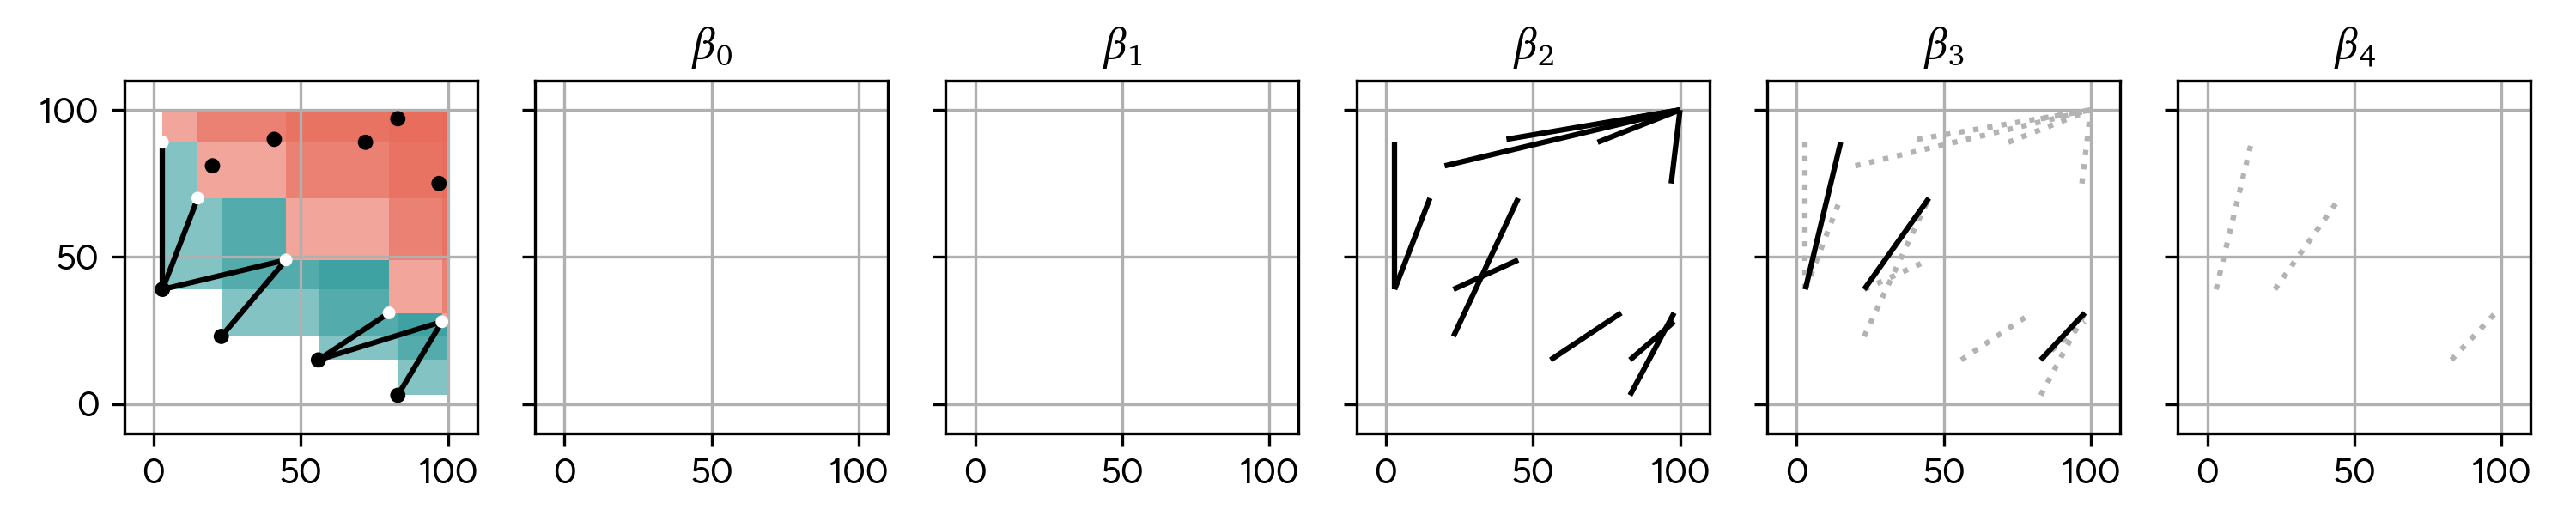
\includegraphics[width=\textwidth]{figs/cokerhooks.png}
    \caption{Result of computing the homology of the cokernel complex; compare with \cref{F:lowerhooks}.}
    \label{F:cokerhooks}
  \end{subfigure}
  \\
  \begin{subfigure}{.4\textwidth}
    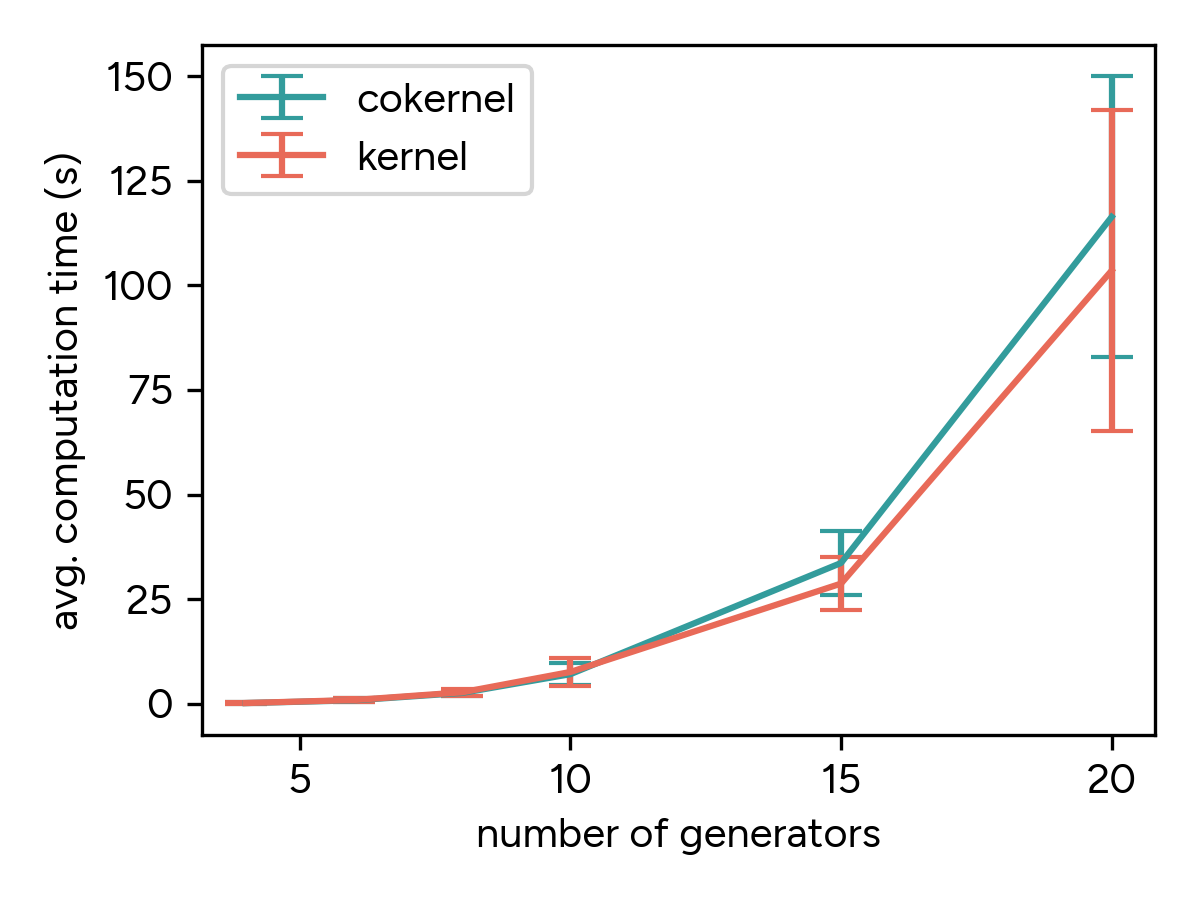
\includegraphics[width=\textwidth]{figs/dev_time.png}
    \caption{Average (of $5$ runs) time to compute relative Betti diagrams with respect to the number of generators.}
    \label{F:dev-time}
  \end{subfigure}
  \hfill
  \begin{subfigure}{.6\textwidth}
    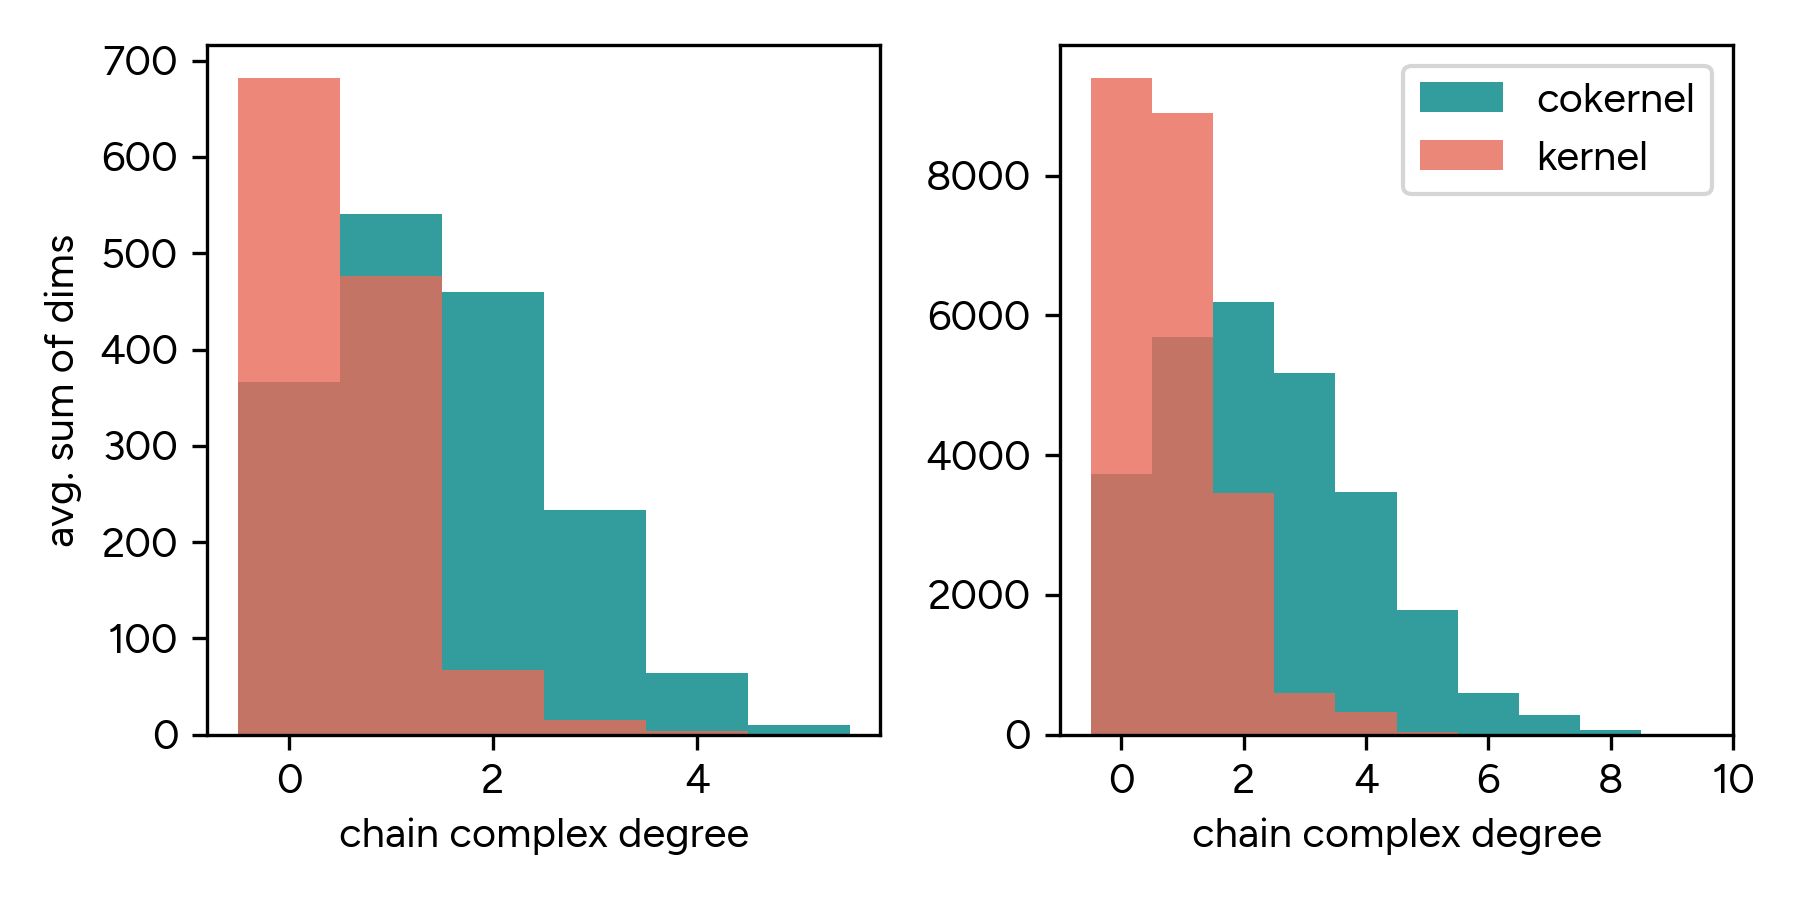
\includegraphics[width=\textwidth]{figs/dev_hist.png}
    \caption{Average (of $10$ runs) sum of dimensions per degree in the Koszul complex of kernels and cokernels for randomly generated persistence modules with $5$ (left) and $10$ (right) generators.}
    \label{F:dev-hist}
  \end{subfigure}
  \caption{Results of the cokernel approach to computing Betti diagrams relative to lower hooks.}
  \label{F:coker-results}
\end{figure}

% \section{Stabilized relative Betti numbers}  % I've kind of avoided defining stabilized ranks

% at IML, with Claudia Landi, Bjørnar Gullikstad Hem, Daniel Tolosa, Berat Geven \ir{surely I don't cite these names, or maybe this result...}

% In \cite{CGRST2024} the authors develop the theory of relative homological algebra for (multiparameter) persistence modules. In particular, given a collection $\mathcal{P}$ of ``simple'' persistence modules, we can define a minimal relative projective resolution of a module $M$ as
% \[
% \cdots \to F_1 \to F_0 \to M \to 0
% \]
% where each $F_i$ is of the form $\bigoplus_{A \in \mathcal{P}} A^{\oplus \beta_i^{\mathcal{P}}M(A)}$, with $\beta_i^{\mathcal{P}} M \colon \mathcal{P} \to \mathbb{N}$ giving the multiplicity of each module $A$ of $\mathcal{P}$ in $F_i$. These multiplicities are the \emph{relative Betti numbers}, and the paper gives a strategy to efficiently compute them for certain collections $\mathcal{P}$, using (local) Koszul complexes. When $\mathcal{P}$ is the collection of free modules, then the relative Betti numbers are exactly the standard Betti numbers; in the notation the $\mathcal{P}$ is omitted.

% Separately, in \cite{GafvertChacholski2021}, the authors show that the hierarchical stabilization of the standard $0^{\text{th}}$ Betti number $\beta_0 M$ is NP-hard to compute, while also giving a strategy for computing them (not so efficiently). We then had two broad research directions:
% \begin{enumerate}
% \item understand the algorithm for computing stabilized $\beta_0$;
% \item understand the stabilized relative $\beta_0$.
% \end{enumerate}
% We focused on the second direction, where we managed to prove the following.

% \paragraph{Result.} If $\{\text{free}\} \subseteq \mathcal{P} \subseteq \{\text{single-source}\}$, where single-source modules are those with a single generator, then $\widehat{\beta_0^{\mathcal{P}} M} \geq \widehat{\beta_0 M}$ for all persistence modules $M$.

% That is, given a fixed noise system, if the collection $\mathcal{P}$ contains all free modules and only contains single-source modules, then the stabilized relative $\beta_0$ is always greater than the stabilized standard $\beta_0$.

% \ir{proof?}

% \section{Dual poset elements for Koszul complexes}

% with Wojciech Chachólski and Marve Grönblad Vesterinen.

% This was a Master's thesis. We define a notion of \term[dual element]{dual elements} for lattices $I$ such that the Betti diagrams of the minimal projective and injective resolutions of a functor over $I$ are dual in some sense.

\section{Space of rank functions}

With Wojiech Chachólski, Andrea Guidolin, Christina Kapatsori, Woojin Kim, Francesca Tombari.

The rank function $\rank V$ of a persistence module $V$ over a poset $I$ (\cref{!D:rank-function}) satisfies the following inequalities. For all chains $a \leq b \leq c \leq d$ in $I$,
\begin{enumerate}
  \item (\term{monotonicity}) $\rank V(a \leq d) \leq \rank V(b \leq c)$, and
  \item (\term{chain-supermodularity}) $\rank V(a \leq d) + \rank V(b \leq c) \leq \rank V(a \leq c) + \rank V(b \leq d)$.
\end{enumerate}
The name \term{chain-supermodularity} comes from \textbf{supermodularity}, a notion studied in probability and order theory \cite{PromislowYoung2005}. Monotone, chain-supermodular functions form a positive convex cone. The broad aim of this project is to study this cone and investigate if we can express rank functions as convex combinations of extremal rays.

As a first step, we study \term{chain-modular} functions, which satisfy the chain-supermodularity condition but with an equality instead of inequality. An interesting question is: which functors have rank functions that are chain-modular? We give some characterizations of the space of chain-modular functions and functors depending on the structure of the underlying poset $I$.
\ir{REVIEW: When $I$ has trivial $H^1$...}

\section{Rank-based noise systems for multiparameter persistence}

With Håvard Bakke Bjerkevik, Andrea Guidolin, and Martina Scolamiero.

For $p \geq n + 1$ and $V \colon \R^n \to \Vect$ an $n$-dimensional persistence module, consider the following integral:
\[
  \| V \|_{p} \coloneq \left( \int_{\vec{x} \leq \vec{y} \in \Omega} p (p - 1)(y_1 - x_1)^{p - n - 1} \rank V(\vec{x} \leq \vec{y}) \right)^{\frac{1}{p}},
\]
where $\Omega \coloneq \{(\vec{x}, \vec{y}) \in (\R^n)^2 \mid \vec{x} \leq \vec{y}\}$ for the product order on $\R^n$.

Following Papers \ref{PC:AGRS2025} and \ref{PC:GRRS2026}, we show the following:

\begin{proposition}
  Let $p \in [n + 1, \infty)$. The $p$-norm on $n$-dimensional persistence modules defines in amplitude. In other words, the $p$-norm defines a noise system.
\end{proposition}

\begin{proof}[Sketch of proof]
  The first, easier short exact sequence axiom (see \cref{!D:noise-system}) comes from [Paper \ref{PC:GRRS2026}, Proposition 4.9], as in the one-dimensional case.

  To prove the second, harder short exact sequence axiom, we proceed as follows. We restrict the rank function of $V$ to lines in $\R^n$ parameterized as $\ell \colon t \mapsto t \vec{a} + \vec{b}$, where $\vec{a} = (1, a_2, \ldots, a_n)$ and $\vec{b} = (0, b_2, \ldots, b_n)$. Then we parameterize our pairs of points $(\vec{x}, \vec{y})$ in $\Omega$ by scalars $s$ and $t$ in $\R$:
  \[
    \vec{x} = s \vec{a} + \vec{b}, \qquad \vec{y} = t \vec{a} + \vec{b}.
  \]
  Then we have the change of parameters
  \begin{equation}
  \label{Eq:reparam}
    \begin{aligned}
      \| V \|_p^p & = \int_{(\vec{x} \leq \vec{y}) \in \Omega} p (p - 1) (y_1 - x_1)^{p - n - 1} \rank V(\vec{x} \leq \vec{y}) \\
      & = \int_{\vec{a} \geq 0} \int_{\vec{b} \in \R^n} \int_{s = -\infty}^{+\infty} \int_{t = s}^{+\infty} p (p - 1) (t - s)^{p - 2} \rank V(\vec{p}, \vec{q}) \text{d}t \text{d}s \text{d}\vec{b} \text{d}\vec{a},
    \end{aligned}
  \end{equation}
  where the proof relies on the computation of the Jacobian of the change of parameters:
  \[
    J_\varphi = \bordermatrix{%
    & s & t & a_2 & b_2 & a_3 & b_3 & \cdots \cr
    p_1 & 1 & 0 \cr
    q_1 & 0 & 1 \cr
    p_2 & a_2 & 0 & s & 1 \cr
    q_2 & 0 & a_2 & t & 1 \cr
    p_3 & a_3 & 0 &&& s & 1 \cr
    q_3 & 0 & a_3 &&& t & 1 \cr
    \vdots & \vdots & \vdots &&&&& \ddots
    }
  \]
  In particular, we have $|\det J_\varphi| = (t - s)^{n - 1}$.

  For a given line $\ell \colon t \mapsto t \vec{a} + \vec{b}$, we apply the result that the $p$-norm gives a noise system in the one-dimensional case. In particular, given a short exact sequence $0 \to U \to V \to W \to 0$ of $n$-dimensional persistence modules, we use the characterization of $p$-norms as integrals of the rank function [Paper \ref{PC:GRRS2026}, Proposition 4.7] to obtain the following triangular inequality:
  \begin{align*}
    & \left(\int_{s = -\infty}^{+\infty} \int_{t = s}^{+\infty} p (p - 1) (t - s)^{p - 2} \rank V(\vec{x} \leq \vec{y}) \text{d}t \text{d}s\right)^{\frac{1}{p}} \\
    & \leq \left(\int_{s = -\infty}^{+\infty} \int_{t = s}^{+\infty} p (p - 1) (t - s)^{p - 2} \rank U(\vec{x} \leq \vec{y}) \text{d}t \text{d}s\right)^{\frac{1}{p}} \\
    & \hspace{2em} + \left(\int_{s = -\infty}^{+\infty} \int_{t = s}^{+\infty} p (p - 1) (t - s)^{p - 2} \rank W(\vec{x} \leq \vec{y}) \text{d}t \text{d}s\right)^{\frac{1}{p}}.
  \end{align*}
  Let
  \[
    f(\vec{a},\vec{b}) \coloneq (\int_{-\infty}^\infty \int_s^\infty p (p - 1) (t-s)^{p - 2} \rank U(\vec{x} \leq \vec{y}) dt ds)^{\frac 1p},
  \]
  and define $g$ and $h$ similarly. Then the previous equations rewrites as $f \leq g + h$.

  We can apply Minkowski's inequality, which states that $(\int (f + g)^p)^{\frac 1p} \leq (\int f^p)^{\frac 1p} + (\int g^p)^{\frac 1p}$ holds for $1 \leq p < \infty$. We get
  \[
    (\int_{\vec{a}} \int_{\vec{b}} f(\vec{a}, \vec{b})^p d\vec{b} d\vec{a})^{\frac{1}{p}} \leq (\int_{\vec{a}} \int_{\vec{b}} g(\vec{a}, \vec{b})^p d\vec{b} d\vec{a})^{\frac{1}{p}} + (\int_{\vec{a}} \int_{\vec{b}} h(\vec{a}, \vec{b})^p d\vec{b} d\vec{a})^{\frac{1}{p}}.
  \]
  By \eqref{Eq:reparam}, this exactly says that
  \[
    \| V \|_p \leq \| U \|_p + \| W \|_p,
  \]
  and this is the hard axiom of noise systems.
\end{proof}

% \section{Matching costs}

% $\| \mu_1 \bullet \mu_2 \|_p \leq \| \mu_1 \|_p \| \mu_2 \|_p$ ?

\section{\texorpdfstring{$p$}{p}-norms of extensions}

This is the content of Hugo Åkesson's Masters thesis \cite{Åkesson2023}, which I co-supervised with Wojciech Chachólski.

Let $V$ and $W$ be persistence modules. An \term[extension]{extension of $V$ by $W$} is a persistence module $E$ that fits into a short exact sequence
\[
  0 \to W \to E \to V \to 0.
\]
We denote by $\Ext(V, W)$ the collection of extensions up to isomorphism (a morphism of extensions is one that commutes with the maps from $W$ and to $V$), and it turns out that this collection forms a vector space.
The question that Åkesson studied is: what is the maximal $p$-norm of an extension? We have results if $W$ is a single bar:

\begin{theorem}[{\cite[Theorem 3.1]{Åkesson2023}}]
\label{T:antichain-extensions-1}
  Let $V$ be a tame persistence module and $[a, b)$ an interval of $\R$. Write
  \[
    F^{ab}(V) \coloneq \{(c, d) \in \cc{D}(V) \mid a < c \leq b < d\}.
  \]
  Then there exists explicitly constructed bijection
  \[
    \psi \colon \{ \text{antichains in } F^ab(V) \} \cong \barcode(\Ext(\K_{[a, b)}, V)),
  \]
  where antichains are defined in [Paper \ref{PC:CGRST2024}, \textsection 4.6] and $\barcode(-)$ is the set of barcodes of elements of the argument.
\end{theorem}

Moreover, we can equip antichains with a partial order $\preceq$ (see again [Paper \ref{PC:CGRST2024}, \textsection 4.6]) such that the following result holds.

\begin{theorem}[{\cite[Theorem 3.2]{Åkesson2023}}]
\label{T:antichain-extension-2}
  We use the notations of \cref{T:antichain-extensions-1} and fix $p \in [1, \infty]$. The function $A \mapsto \| \psi(A) \|_p$ from antichains in $F^{ab}(V)$ to $p$-norms is monotone. In other words, for antichains $A$ and $B$ in $F^{ab}$,
  \[
    A \preceq B \quad \Rightarrow \quad \| \psi(A) \|_p \leq \| \psi(B) \|_p.
  \]
\end{theorem}

Notably, the poset of antichains of $F^{ab}$ has a greatest element, the antichain of maximal elements of $F^{ab}$. By \cref{T:antichain-extension-2}, the bijection $\psi$ sends this antichain to the extension barcode with the greatest $p$-norm.

When $W$ is arbitrary, Åkesson provides a recursive formula \cite[Theorem 4.1]{Åkesson2023}: if $W = W_1 \oplus W_2$ with $\Ext(W_1, W_2) = 0$ (this is always possible), then
\begin{equation}
\label{Eq:recursive-extension}
  \barcode(\Ext(W, V)) = \bigcup_{B \in \barcode(\Ext(W_2, V))} \barcode(\Ext(W_1, \cc{V}(B))),
\end{equation}
where $\cc{V}(B)$ is a persistence module with barcode $B$. This gives an iterative strategy for computing $\barcode(\Ext(W, V))$: sort the bars of $W$ compatibly with the product order on the start- and endpoints, set $W_2$ equal to the first bar and $W_1$ to the sum of the rest: by construction, we get $\Ext(W_1, W_2) = 0$.

It is still an open problem to determine the extension with largest $p$-norm. This is useful, for example, in the study of the noise system axioms for $p$-norms.

\section{Pair degree}

Following discussions with Emil Horobeț.

In Papers \ref{PC:GLRS2025} and \ref{PC:Ren2026}, we defined notions of algebraic critical points, and bounded their number. The number of algebraic critical points, in the complex setting, could define a new numerical invariant that generalizes the Euclidean distance degree and the bottleneck degree. Here we sketch its definition:

\begin{definition}
  Let $X$ and $Y$ be complete intersections defined by polynomials $\vec{p}$ and $\vec{q}$, respectively. We define the \term[pair degree]{pair degree of $X$ and $Y$} to be the cardinality of the set $C_k(\vec{p}, \vec{q})$ of algebraic critical points of the distance function $\dist_Y\big|_X$ (see Paper \ref{PC:Ren2026}, Definition 3.3.2).
\end{definition}

\ir{REVIEW: Say a bit more}
% !TEX root = ../thesis-main.tex

\chapter{Papers and contributions}

\addtocontents{toc}{\protect\setcounter{tocdepth}{0}}

\papersection{CGRST2024}

In this paper, we study persistence modules over a finite poset $(I, \mathord{\leq})$ using the functorial perspective (\cref{SS:functor}). We extend the results of \cref{S:persistent-homological-algebra} to the \term[relative homological algebra]{relative homological case}. Instead of approximating functors over $I$ by projective resolutions, where each term is a sum of free functors, we approximate them by other ``simple'' functors. Given a collection $\cc{P}$ of such simple functors, we define $\cc{P}$-exactness, $\cc{P}$-projectives, $\cc{P}$-covers, and $\cc{P}$-resolutions, which are the relative versions of the ``absolute'' notions defined in \cref{S:persistent-homological-algebra}. A \term[$\cc{P}$-free]{$\cc{P}$-free functor} is a functor that is isomorphic to a direct sum of elements of $\cc{P}$. The collection $\cc{P}$ is then \term{acyclic} if every $\cc{P}$-projective is $\cc{P}$-free. Under this condition, we can then define Betti diagrams relative to $\cc{P}$.

The principal result of this paper is that, under reasonable conditions on $\cc{P}$, we can compute the relative Betti diagrams using local Koszul complexes. First, assume that the collection $\cc{P}$ is parameterized by a functor $\cc{T} \colon (J, \mathord{\preceq})^{\op} \to \Fun(I, \Vect)$ where $(J, \mathord{\preceq})$ is a finite upper semilattice (\ir{ref}) and $\cc{P} = \{\cc{T}(a) \mid \cc{T}(a) \neq 0, \; a \in J\}$. The parameterization functor $\cc{T}$ is \term{thin} if, for all $a \preceq b$ in $J$, the space of natural transformation $\Nat(\cc{T}(b), \cc{T}(a))$ is of dimension at most $1$. In this case, the collection $\cc{P}$ is acyclic, and so we can talk about Betti diagrams relative to $\cc{P}$: given a functor $M \colon I \to \Vect$ and an element $a \in J$ such that $\cc{T}(a) \neq 0$, we denote by $\beta_{\cc{P}}^d M(a)$ the multiplicity of $\cc{T}(a)$ in the $d^{\th}$ term of the minimal $\cc{P}$-projective resolution of $M$.

Given a functor $M \colon I \to \Vect$, we define the functor indexed by $J$
\[
  \cc{R} M \colon \left\{ \begin{array}{ccc}
    J & \to & \Vect \\
    a & \mapsto & \Nat(\cc{T}(a), M).
  \end{array} \right.
\]
The main result is the following.

\begin{theorem}[\ir{Corollary 5.20, Paper A}]
  Let $(J, \mathord{\preceq})$ be an upper semilattice and $\cc{T}$ a thin parameterization functor. Assume that
  \begin{enumerate}
    \item the set $\{a \in J \mid \cc{T}(a) = 0\}$ is closed under joins, and
    \item for all $a, b$ in $J$, if $b$ is minimal $\succeq a$ such that $\Nat(\cc{T}(b), \cc{T}(a)) = 0$, then $\cc{T}(a) = 0$.
  \end{enumerate}
  Then, for all functors $M \colon I \to \Vect$, all $a$ in $J$ such that $\cc{T}(a) \neq 0$, and all $d \geq 0$,
  \[
    \beta_{\cc{P}}^d M(a) = \dim H_d(\cc{K}_a \cc{R} M).
  \]
\end{theorem}

In other words, under the listed conditions, we can compute the Betti diagrams relative to $\cc{P}$ using the standard Koszul complexes defined on $\cc{R} M \colon J \to \Vect$.

The paper ends with an extensive list of examples of collection $\cc{P}$ and parameterization functors $\cc{T}$ where the conditions of the theorem hold. This includes examples that have been studied in previous works, including \textbf{rectangles}, \textbf{lower hooks} \cite{BOO2025}, and \textbf{single-source spread modules} \cite{BBH2024}. In fact, this work was in part motivated by the study of exact structures for persistence modules, in particular relative to lower hooks, in \cite[Section 4]{BOO2025}. We have also implemented the computation of Betti diagrams relative to lower hooks in Python \cite{lowerhooks}.

\ir{figure}

Related: decompositions of rank functions \ir{put this elsewhere}

\subsection*{Erratum}

Thank you to Tada Shunsuke for pointing out the following mistake. In \textsection 4.4, we write that a functor $F \colon J \to \Vect$ is isomorphic to a subfunctor of $\K_J$ if, and only if, $F$ is a filtration and $\dim F(a) \leq 1$ for every $a$ in $J$. This does not hold in all generality: consider the functor $F$ defined by
\[
  \begin{tikzcd}
    \K
      \arrow[r, "1"]
      \arrow[d, "1" swap]
    & \K
    \\
    \K
    & \K
      \arrow[l, "1"]
      \arrow[u, "\lambda" swap]
  \end{tikzcd}
\]
where $\lambda \in \K \setminus \{0, 1\}$. Then $F$ is a filtration with pointwise dimension at most $1$, but is not isomorphic to a subfunctor of $\K_J$. As a correction, we restrict the claim to the case where $J$ is an upper semilattice. There is no impact on the rest of the paper. \ir{right?}

\subsection*{Contributions}

In this paper I co-wrote the main results, was the main contributor to the analysis of examples in the last section, and wrote the software \texttt{lowerhooks} \cite{lowerhooks} that applies our theoretical results to the specific case of lower hooks.

CRediT classification: \textbf{Isaac Ren:} conceptualization (equal), formal analysis (equal), software (lead), visualization (lead), writing - original draft preparation (equal), writing - review \& editing (equal).

\papersection[shorttitle={Algebraic Wasserstein distances...}]{AGRS2025}

In this paper, we define algebraic $p$-Wasserstein distances for tame persistence modules, proving that the sequence of collections $\cc{S} = \{\cc{S}_\varepsilon\}_{\varepsilon \geq 0}$ of \cref{SS:algebraic-wasserstein} is indeed a noise system. This is an alternate proof to that of \cite{SkrabaTurner2023}, \ir{a preprint that is being rewritten at the time of publication (like honestly what do I say here)}.

The difficult noise system axiom to prove is the exact sequence, and specifically the following lemma:

\begin{lemma}[\ir{Lemma 4.15, Paper B, simplified}]
\label{L:triangular-ineq}
  Let $0 \to U \xrightarrow{f} V \xrightarrow{g} W \to 0$ be an exact sequence of tame persistence modules, and $p \in [1, \infty]$ a number. Then
  \[
    \| V \|_p \leq \| U \|_p + \| W \|_p.
  \]
\end{lemma}

Our proof strategy is to observe that the morphism $f$ is a monomorphism and that $W \cong \coker f$, and then study cases where the $p$-norm of $\coker f$ is easy to compute. We identify the following notion.

\begin{definition}
  A morphism $f \colon V \to W$ of tame persistence modules is \term{bar-to-bar} when there exists a matrix representation of $f$ such that each row and column has at most one nonzero coefficient.
\end{definition}

In other words, for a bar-to-bar morphism, there exist barcode decompositions of the domain and codomain such that each bar of the domain maps to at most one bar of the codomain. The key result is the following.

\begin{theorem}{\ir{Theorem 3.14}}
  Let $f \colon V \hookrightarrow W$ be a monomorphism of tame persistence modules. Then there exists a bar-to-bar monomorphism $f_b \colon V \hookrightarrow W$ such that $\| \coker f_b \|_p \leq \| \coker f \|_p$ for all $p \in [1, \infty]$.
\end{theorem}

Moreover, we observe that \cref{L:triangular-ineq} \ir{is easy to show for bar-to-bar monomorphisms as the triangular inequality on the vectors of bar lengths, and this gives the triangular inequality...}

\ir{isometry result}

In this paper, we also introduce \ir{extra parameterization on $p$-Wasserstein distances: an extra number $q$ for combining costs (combinatorial def?) and a lifetime function to weight bars by their position. Hierarchical stabilization,which we can compute explicitly. We then study case of brain arteries, where we can learn optimal parameterizations for a classification task}


\papersection[misctext=To be submitted]{GRRS2026}

Induced matchings.

Applications: interpretability?

\papersection[shorttitle={Morse theory of Euclidean distance functions...}, misctext=Submitted]{GLRS2025}

Distance function as continuous selection: not obvious, needs to be shown, cite result.

Generic nondegeneracy between hyperplanes

\papersection[shorttitle={Nondegeneracy of distance functions...}, misctext=To be submitted]{Ren2026}

case of complete intersections

\addtocontents{toc}{\protect\setcounter{tocdepth}{1}}

\printbibliography[title=References,heading=bibintoc]

% ==== PAPERS ====

\part{Papers}
\label{Part:papers}
\newrefsection% Reset the bibliography
\addtocontents{toc}{\protect\setcounter{tocdepth}{0}}% https://www.reddit.com/r/LaTeX/comments/1khta4d/comment/mr9hxeb/

\papertitlepage[color=light blue]{CGRST2024}

% 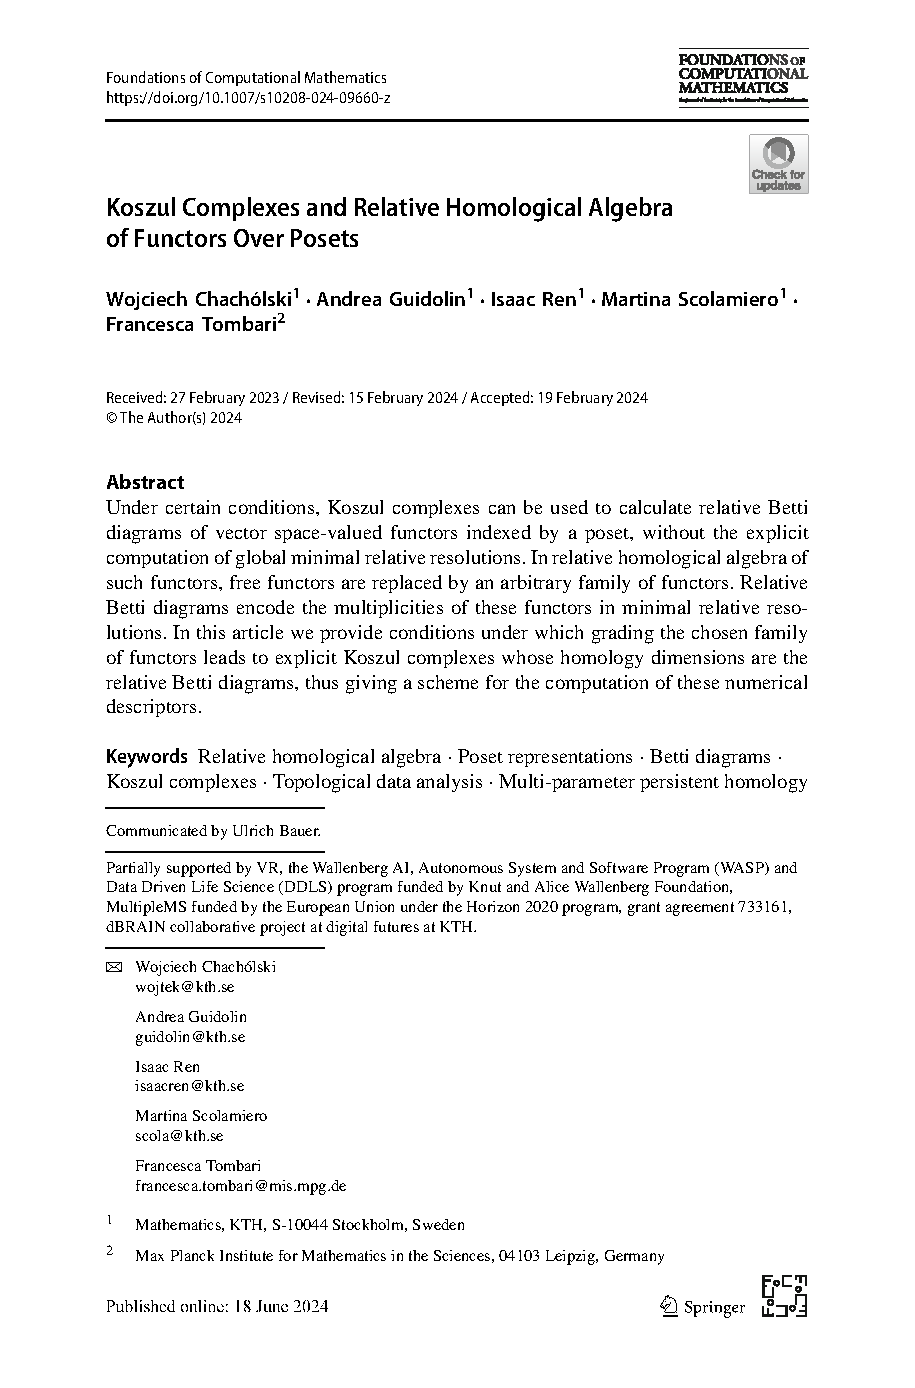
\includepdf[pages=-]{papers/CGRST2024}

\papertitlepage[color=light blue]{AGRS2025}

% 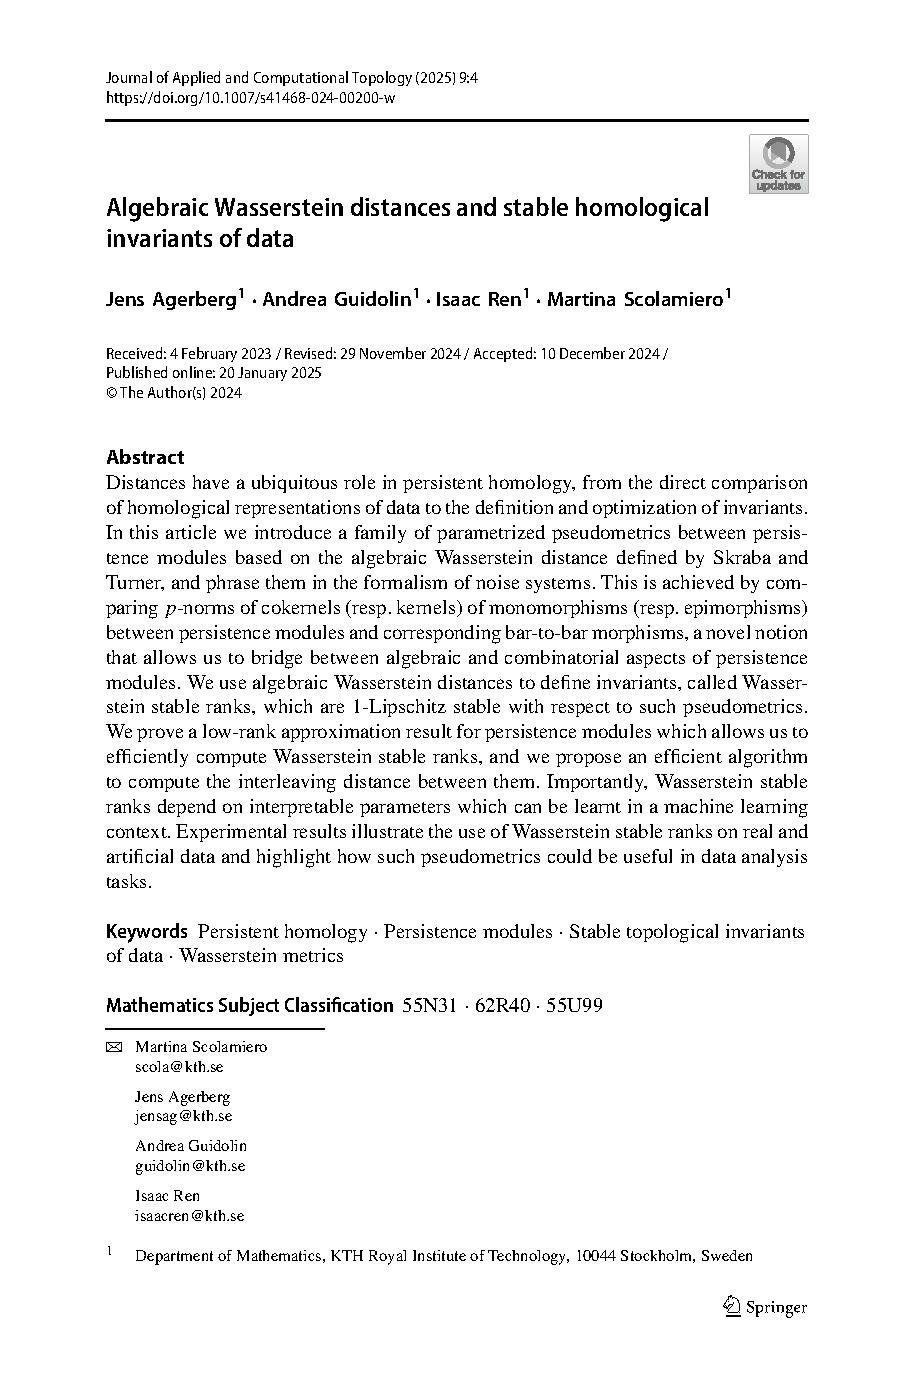
\includepdf[pages=-]{papers/AGRS2025}

\papertitlepage[color=light blue,misctext=To be submitted]{GRRS2026}

\paperchapter{GRRS2026}

\papertitlepage[color=light blue,misctext=Submitted]{GLRS2025}

\paperchapter{GLRS2025}

\begin{paperabstract}%[.9\textwidth]% default value
This abstract is in a \texttt{paperabstract} environment. Lorem ipsum dolor sit amet!
\end{paperabstract}

The usual approach to including papers is to include PDFs. \texttt{kthpq-thesis} does not provide any tools for that; use your favorite package or external method. If you wish to include your paper's \TeX{} code directly in the thesis, add the line
\begin{verbatim}
\paperchapter[Short title]{REF}
\end{verbatim}
where \texttt{REF} is the bibliography reference for the paper, and \texttt{Short title} is the title that will appear in the headers.

\section{Introduction}

text

\papertitlepage[color=light blue,misctext=To be submitted]{Ren2026}

\paperchapter{Ren2026}

% ---- Back matter ----

\backmatter

\begin{colophon}[.5\textwidth]
\footnotesize
\setlength{\parindent}{1pc}
\noindent This thesis is set in Figtree, Georgia, Fira Code, and XCharter-Math.

Headings and some short body text are set in Figtree, designed by Eric Kennedy in 2022. Minimalist yet friendly, Figtree is a geometric sans serif face made for the digital age.

The body text face is Georgia, designed by Matthew Carter and hinted by Thomas Rickner in 1993. Georgia is a serif face in the Scotch Roman style designed to be legible on low-resolution screens, but its elegant forms are equally appreciated at higher resolutions and in print.

The monospace face is Fira Code, designed Nikita Prokopov in 2019. It is based on the Fira Mono typeface by Carrois Apostrophe and features an extensive set of ligatures for many programming languages.

The mathematical text is set in XCharter-Math, designed and maintained by Daniel Flipo for \TeX. This OpenType math font borrows and derives its symbols from XCharter, designed and maintained by Michael Sharpe and itself derived from Matthew Carter's Bitstream Charter (a predecessor to Georgia), as well as MathDesign by Paul Pichaureau and Fourier-GUTenberg by Michel Bovani.

\mydinkus

\noindent This thesis was typeset on \today{} by \formattedluatexbanner{} with \LaTeX2e{} (\fmtversion) and \textsf{expl3} (\ExplLoaderFileDate) using the class \href{https://github.com/th-rtyf-re/kthpq-thesis}{\texttt{kthpq-thesis}} written by me!
\end{colophon}

\end{document}